\chapter{Flujo de trabajo y Aplicación Web}

\begin{figure}[H]
    \centering
    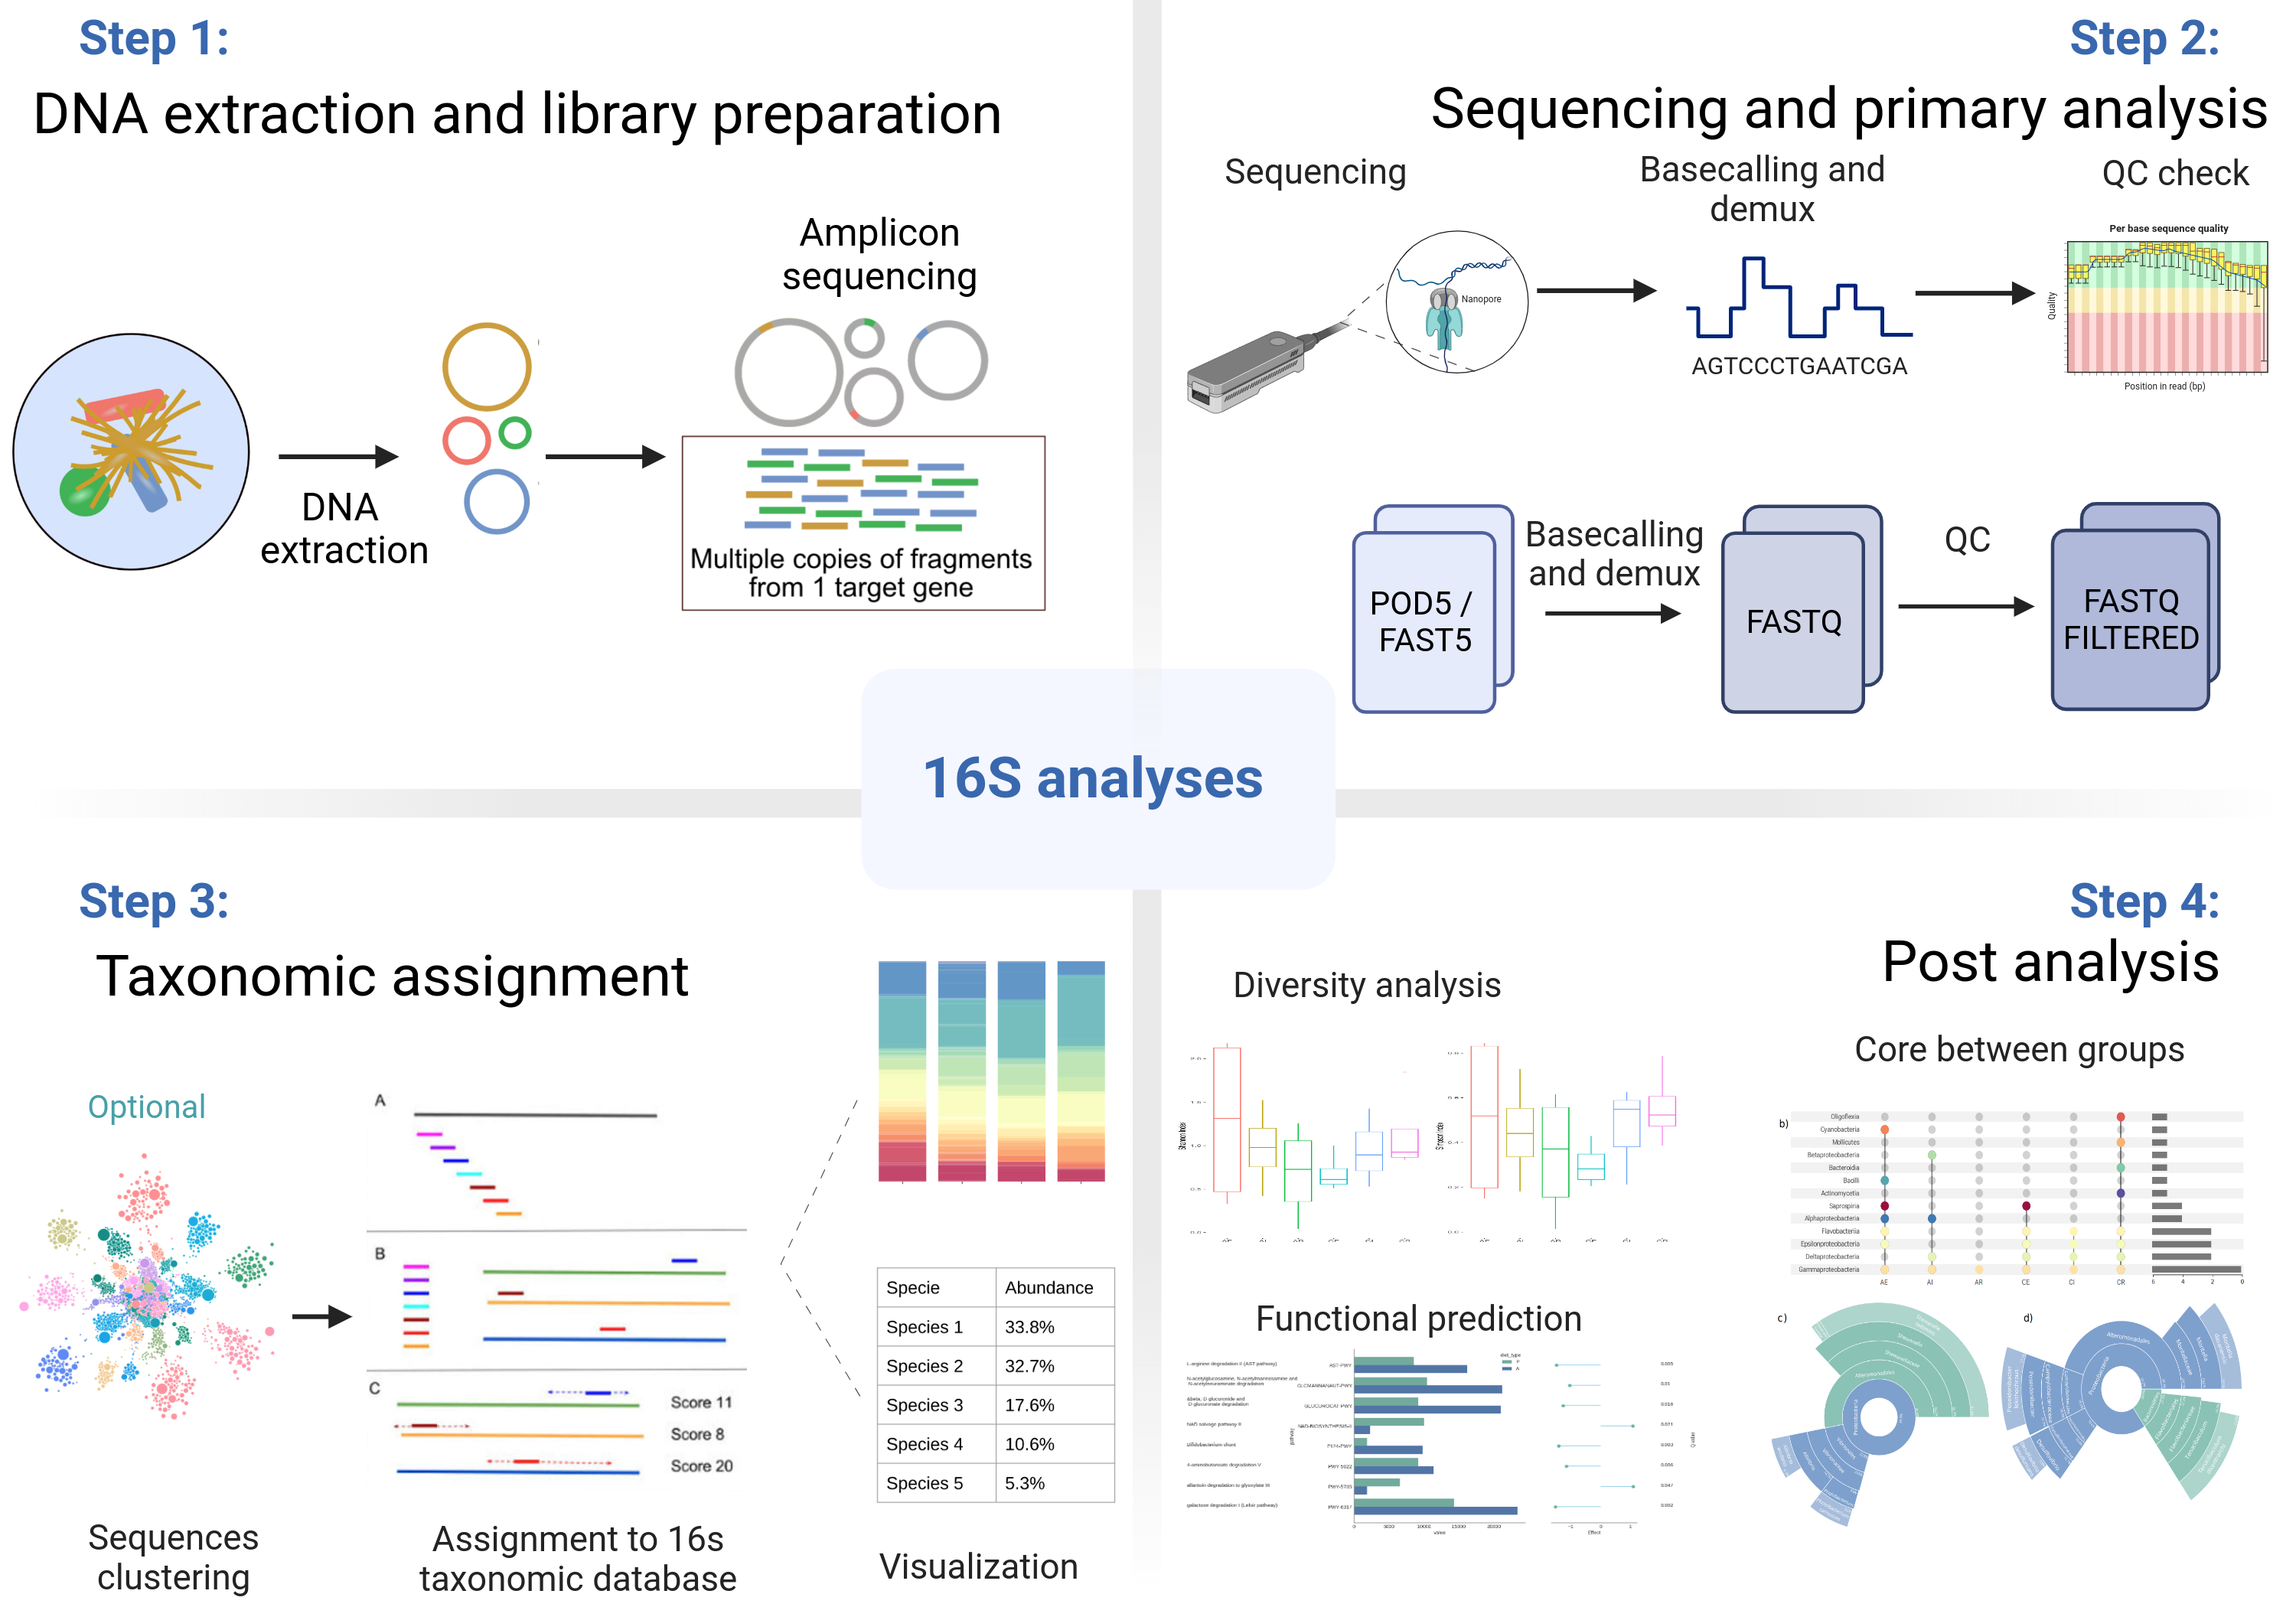
\includegraphics[width=1\linewidth]{images/16s_workflow_schema.jpeg}
    \caption{Flujo de trabajo estándar para la secuenciación y análisis de secuenciaciones del gen 16S}
    \label{fig:16S_workflow}
\end{figure}
\section{Flujo de trabajo}
Se desarrolló un flujo de trabajo automatizado en Nextflow que permite el análisis y caracterización de secuencias del gen 16S obtenidas mediante Oxford Nanopore. El flujo de trabajo está desarrollo de manera modular permitiendo que el usuario pueda personalizar su ejecución, agregando o quitando subworkflows o módulos según sus necesidades. Cuenta con los siguientes módulos:
\begin{itemize}
    \item Basecalling y demultiplexacion:
    \item Control de calidad:
    \item Asignación taxonómicas:
    \item Caracterización de la comunidad microbiana:
\end{itemize}
%para el preprocesamiento de las secuencias, la identificación de las secuencias mediante BLAST/mmseqs, la identificación de comunidades microbianas mediante la base de datos de 16S de Genbank, el calculo de índices de diversidad, la identificación de genes funcionales mediante PICRUSt2, y el análisis estadístico de los resultados funcionales mediante Aldex2 y Lefse. También cuenta con un modulo de visualización de las asignaciones taxonómicas mediante el uso de script personalizados hechos en python.
\hl{Desarrollo de contenedores o conda enviroments}
\begin{figure}[H]
    \centering
    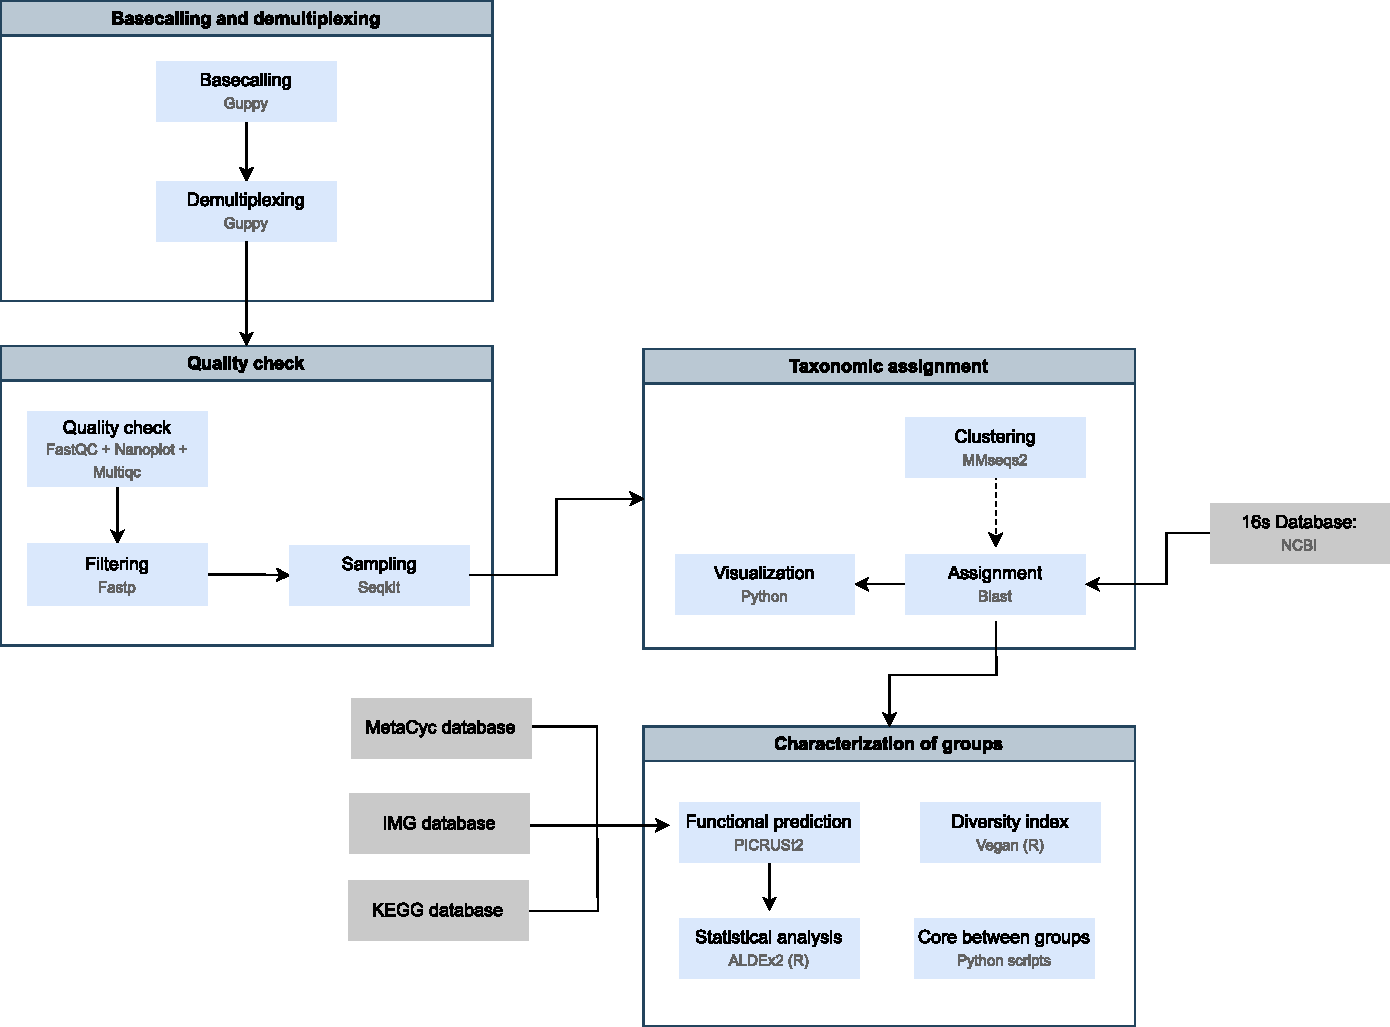
\includegraphics[width=1\linewidth]{images/pipeline.pdf}
    \caption{Bioinformatics pipeline}
    \label{fig:pipeline}
\end{figure}
El flujo de trabajo cuenta con parámetros generales que son independientes de los módulos:
\begin{itemize}
    \item stage: Subworkflow a ejecutar. Puede contener los siguientes valores:
          \begin{itemize}
              \item All\_without\_basecalling: Ejecutar todo el flujo de trabajo sin incluir basecalling y demultiplexación.
              \item All\_with\_basecalling: Ejecutar todo el flujo de trabajo incluyendo el proceso de basecalling y demultiplexacion.
              \item Preprocessing: Ejecutar solo el subworflow de preprocesamiento
              \item TaxonomyAssignament: Ejecutar el modulo de asignación taxonomca.
              \item Visualization: Ejecutar solo el subworkflow de visualización de gráficos
              \item Functional: Ejecutar solo el subworkflow de predicion funcional
              \item Diversity: Ejecutar solo los modulos de indices de diversidad

          \end{itemize}
    \item input:
    \item samples.csv:
\end{itemize}

\subsection{Ejecución de flujo de trabajo completo}
\hl{hacer un esquema de los casos del uso, que el usuario puede comenzar con fastq, pod5, o hacer solo los graficos, etc}
\subsection{Control de calidad}
Este módulo primero se encarga de realizar un control de calidad a las secuencias mediante las herramientas FastQC y Nanoplot.  Posteriormente, se eliminan secuencias de baja calidad y secuencias no pertenecientes al gen 16s (basado en el tamaño de la lectura). Para esto, se utiliza el software Fastp \cite{} que permite realizar las tareas mencionadas anteriormente.

Input:
Output:
Parámetros:


\subsection{FastQC y Nanoplot}
FastQC y Nanoplot reciben como input el archivo FASTQ a procesar y entrega como output un archivo HTML con el reporte del control de calidad. Este reporte será utilizado para integrar la información de este proceso en el reporte de MultiQC.
En el flujo de trabajo ambas herramientas se utilizarán dos veces, una vez con el archivo FASTQ raw y otra vez con el archivo FASTQ preprocesado.
\subsection{Fastp Parametros}

\begin{itemize}
    \item q 15
    \item cut\_mean\_quality 15
    \item length\_required 1000
    \item length\_limit 2200
    \item disable\_adapter\_trimming
    \item disable\_trim\_poly\_g
\end{itemize}

Fastp recibe como input el archivo FASTQ raw y entrega como output el archivo FASTQ preprocesado. De igual manera, entrega un reporte en formato HTML y un reporte en formato JSON, el cual posteriormente será utilizado para integrar la información de este proceso en el reporte de MultiQC.

\subsection{SEQKIT}
Seqkit se utilizará para realizar un subsampleo de la muestra y evitar sesgos a la hora de realizar la caracterización por grupos debido a la cantidad de lecturas de cada muestra. Recibe como input el archivo FASTQ preprocesado.
Posteriormente el archivo subsampleado se transformará a formato FASTA mediante la misma herramienta, y será utilizado para realizar la caracterización de la comunidad microbiana.



\subsection{Asignación taxónomica}
Clustering con MMSEQS
\subsubsection{BLAST}
Para la asignación taxonómica se utiliza BLAST con la base de datos de 16s de Genbank.
\begin{itemize}
    \item -mt\_mode 1
    \item -outfmt "6 qseqid staxids sscinames evalue length pident qcovs"
    \item -evalue 0.001
    \item -max\_target\_seqs 1
\end{itemize}
Para asegurar que las secuencias sean asignadas a la taxonomía correcta, se utiliza un evalue de 0.001 y un porcentaje de identidad mayor a \hl{XX}
EL output de BLAST es un archivo de formato tabular (TSV) que contiene el identificador de la muestra, el id de la taxonomia asociada a la secuencia, el nombre científico de la taxonomía, el valor de evalue, el largo de la secuencia, el porcentaje de identidad y el porcentaje de cobertura de la secuencia.

Mediante TaxonKit se obtiene el linage completo de la taxonomía asignada a la secuencia , y se formatea mediante CSVTk.

\subsubsection{MERGE\_BLAST\_OUT}
Se desarrollo un script en python para resumir la asignación taxonomica obtenida con BLAST de todas las muestras en un solo archivo. Además, se generan archivos por cantidad de lecturas y porcentaje, y por cada categoria taxonomica.

\subsection{Caracterización de la comunidad microbiana}
\subsubsection{Stacked Plots}
Se desarrollo un script en python que grafica las taxonomias en graficos de barras apiladas, permitiendo visualizar la distribución de las taxonomias en las muestras.En caso de que el usuario haya ingresado grupos asignados a cada muestra también se obtendran graficos de barras apiladas de los grupos. Las taxonomías menores a un 1\% (valor por defecto y modificable) se agrupan en una nueva taxonomia llama "Otros" y se muestra en color gris.

\begin{itemize}
    \item --taxonomy\_input\_file: Archivo en formato \hl{csv} donde las columnas son las muestras, las filas las taxonomicas y el valor de abundancia de cada taxonomia en cada muestra en el \hl{centro}.
    \item --annotate\_tax: En caso de ser true se anotara el nombre de la taxonomia y el porcentaje en la barra.
    \item min\_abundance\_annotate: Porcentaje de abundancia maximo para agrupar las taxonomicas en sección de otros
\end{itemize}

\subsubsection{Core Plot}
Se desarrollo un script en python que realiza un grafico circular jerarquico de las taxonomias compartidas entre las muestras.
Este grafico puede realizarse a nivel de grupos (siempre que el usuario hubiera ingresado los grupos en el archivo de metadata), y también se realiza entre todas las muestras.
Input: CSV de taxonomia a nivel de especie por muestra y archivo de linajes.
Output: Grafico circular jerarquico de las taxonomias compartidas entre las muestras en formato PDF
\subsubsection{Indices de diversidad}
shannon simpson chao

\subsubsection{Prediccion Funcional}
La predicción funcional se realiza mediante la herramienta PICRUSt2.

Input:
output:
Picrust2 + aldex + Lefse

\section{Base de datos}


\subsection{Tabla de Usuarios}
\begin{table}[H]
    \begin{tabular}{|l|l|l|l|l|}
        \hline
        campo              & tipo de dato & descripción       & PK & FK \\ \hline
        id                 & int          & ID                & Si & No \\ \hline
        username           & str          & Nombre de usuario & No & No \\ \hline
        fullname           & str          & Nombre completo   & No & No \\ \hline
        email              & str          & Email             & No & No \\ \hline
        hasshed\_password  & str          &                   & No & No \\ \hline
        is\_active         & bool         &                   & No & No \\ \hline
        role\_platform\_id & int          &                   & No & Si \\ \hline
    \end{tabular}
    \caption{Tabla Users}
    \label{tab:db-users}
\end{table}
\subsection{Roles de la plataforma}
\begin{table}[H]
    \begin{tabular}{|l|l|l|l|l|}
        \hline
        campo       & tipo de dato & descripción                         & PK & FK \\ \hline
        id          & int          & ID                                  & Si & No \\ \hline
        name        & str          & Nombre del rol (admin / basic user) & No & No \\ \hline
        description & str          & Descripción del rol                 & No & No \\ \hline
    \end{tabular}
    \caption{Tabla PlatformRole}
    \label{tab:db-platformRole}
\end{table}
\subsection{Projectos}


\begin{table}[H]
    \begin{tabular}{|l|l|l|l|}
        \hline
        campo          & tipo de dato          & descripción                                                                                                                       & FK \\ \hline
        id             & int (PK)              & ID                                                                                                                                & No \\ \hline
        name           & str                   & Nombre del projecto                                                                                                               & No \\ \hline
        description    & str                   & Descripción del proyecto                                                                                                          & No \\ \hline
        samples        & JSON/dict{[}str,any\} & \begin{tabular}[c]{@{}l@{}}Metadata de las muestras. Puede contener como claves: \\ Barcode, Sample, Group, Subgroup\end{tabular} & No \\ \hline
        colaboration   & str                   & ???                                                                                                                               & No \\ \hline
        type\_file\_in & str                   & Tipo de archivo a procesar (POD5, FASTQ, CSV, FASTA)                                                                              & No \\ \hline
        path\_data     & str                   & Ruta en el servidor donde se almacenaran los archivos de entrada                                                                  & No \\ \hline
        status         & str                   & \begin{tabular}[c]{@{}l@{}}Estado del proyecto en ejecución \\ (upload\_data / running / failed / finish)\end{tabular}            & No \\ \hline
        note           & JSON/dict{[}str,any\} & \begin{tabular}[c]{@{}l@{}}Información sobre el proyecto \\ (cantidad de muestras total, procesadas y descartadas)\end{tabular}   & No \\ \hline
        logs           & JSON/dict{[}str,any\} & Logs                                                                                                                              & No \\ \hline
        owner\_id      & int                   & Id del usuario que sube el proyecto                                                                                               & Si \\ \hline
    \end{tabular}
    \caption{Tabla de Proyectos}
    \label{tab:db-projects}
\end{table}

\subsection{Roles del Proyecto}
\begin{table}[H]
    \begin{tabular}{|l|l|l|l|}
        \hline
        campo       & tipo de dato & descripción                               & FK \\ \hline
        id          & int (PK)     & ID                                        & No \\ \hline
        name        & str          & Nombre del rol (leer, escribir, eliminar) & No \\ \hline
        description & str          & Descripción del rol                       & No \\ \hline
    \end{tabular}
    \caption{Tabla de Roles de Proyectos}
    \label{tab:db-role_projects}
\end{table}
\subsection{Roles Projectos y Usuarios}
\begin{table}[H]
    \begin{tabular}{|l|l|l|l|}
    \hline
    campo       & tipo de dato & descripción                                       & FK \\ \hline
    user\_id    & int (PK)     & ID del usuario                                    & Si \\ \hline
    project\_id & int (PK)     & ID del proyecto                                   & Si \\ \hline
    role\_id    & int (PK)     & Rol del usuario dentro del proyecto en especifico & Si \\ \hline
    \end{tabular}
    \caption{Tabla de Roles Proyectos y Usuarios}
    \label{tab:db-role_projects_users}
    \end{table}

\subsection{Resultados}
\begin{table}[H]
    \small
    \begin{tabular}{|l|l|l|l|}
    \hline
    campo                  & tipo de dato           & descripción                                                                                                                                              & FK \\ \hline
    id                     & int                    & ID                                                                                                                                                       & No \\ \hline
    taxonomic\_assignament & JSON/dict{[}str,any{]} & \begin{tabular}[c]{@{}l@{}}Assignación taxonomica por muestra y por nivel taxonómico\\ (especie, genero, familia, orden, clase y filo)\end{tabular}      & No \\ \hline
    functional\_prediction & JSON/dict{[}str,any{]} & \begin{tabular}[c]{@{}l@{}}Resultados de la predicción funcional por muestra y \\ por categoría funcional (EC, Pathways, KO)\end{tabular}                & No \\ \hline
    core                   & JSON/dict{[}str,any{]} & Cantidad de lecturas/porcentaje compartido entre los grupos                                                                                              & No \\ \hline
    basic\_statistics      & JSON/dict{[}str,any{]} & \begin{tabular}[c]{@{}l@{}}Estadísticas básicas de las muestras\\ (Total de lecturas procesadas y sin procesar,\\ calidad y largo promedio)\end{tabular} & No \\ \hline
    diversity              & JSON/dict{[}str,any{]} & \begin{tabular}[c]{@{}l@{}}Calculo de los indices de diversidad\\ (Shannon, Simpson, Chao2)\end{tabular}                                                 & No \\ \hline
    config\_run            & JSON/dict{[}str,any{]} & Parámetros personalizados por el usuario                                                                                                                 & No \\ \hline
    project\_id            & int                    & ID del proyecto                                                                                                                                          & Si \\ \hline
    \end{tabular}
    \caption{Tabla de Resultados}
    \label{tab:db-results}
    \end{table}

\newpage
\section{Aplicación Web}
Se desarrollo una aplicación web mediante Vue3 y FastAPI que permite al usuario subir sus archivos de secuenciación y metadata. 
Con esto el usuario puede abstraerse de tener conocimiento en línea de comando o ejecución de heramientas bioinformaticas y/o flujos de trabajo, 
ya que mediante la interfaz web el usuario solo debe seleccionar los análisis que desea realizar.
La información ingresada por el usuario es guardada en la base de datos y mediante un script se generan los parámetros necesarios para la ejecución del flujo de trabajo.
Una vez el pipeline termina de ejecutarse se escriben los resultados en la base de datos. 
La plataforma lee esta información directa de la base de datos y despliega los resultados en forma de tablas y gráficos en la sección de análisis.

A continuación se detalla cada una de las vistas de la aplicación web y su funcionalidad.
% \subsection{Middleware}
% \subsection{Security}

\subsection{Login}
Al ingresar en la página de Login, el usuario deberá ingresar su nombre de usuario y contraseña.
En caso de que los datos sean correctos será redireccionado a la página de proyectos (Ver sección \ref{projects}).
En caso de que los datos sean incorrectos se mostrará un mensaje de error \textit{“Usuario o contraseña incorrectos”} y deberá ingresar sus credenciales nuevamente.


\begin{figure}[ht]
    \centering
    \begin{subfigure}[b]{0.45\textwidth}
        \centering
        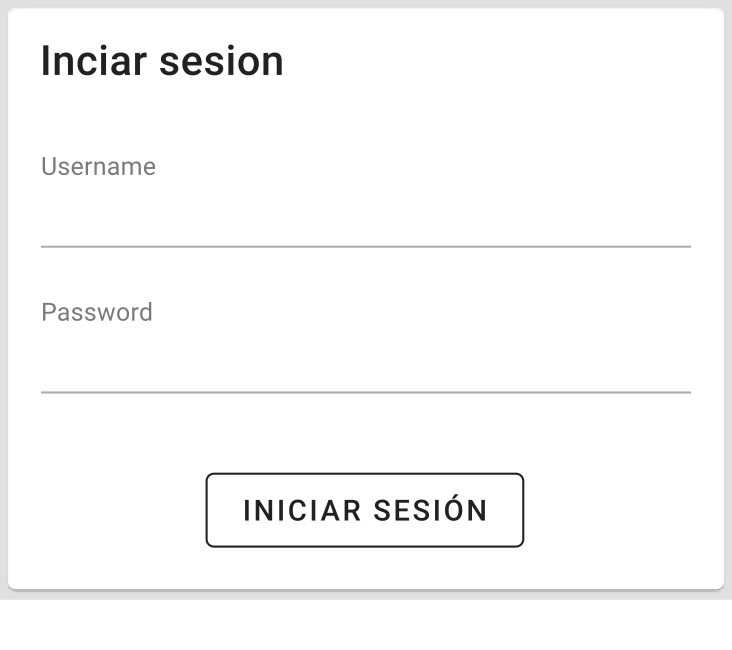
\includegraphics[width=\textwidth]{images/app/login.png}
        \caption{Vista de inicio de sesión por defecto \newline}
        \label{fig:app-login_default}
    \end{subfigure}
    \hfill
    \begin{subfigure}[b]{0.45\textwidth}
        \centering
        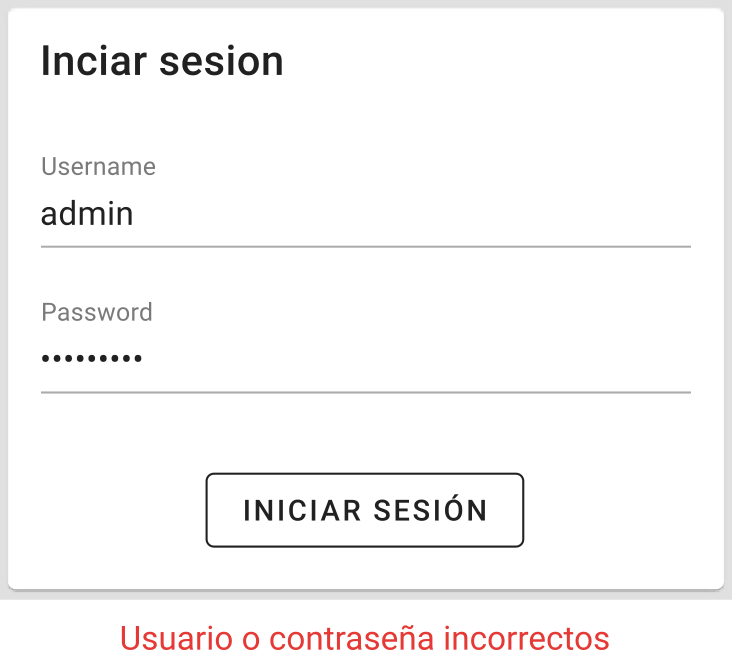
\includegraphics[width=\textwidth]{images/app/login-error.png}
        \caption{Vista de inicio de sesión con mensaje de error al ingresar credenciales inválidas}
        \label{fig:app-login_error}
    \end{subfigure}
    \caption{Vista de Inicio de sesión}
    \label{fig:app-login}
\end{figure}

\hl{Registrarse - vista}
\subsection{Navbar?}

\subsection{Cambio de contraseña}
Una vez que el usuario validó sus credenciales va a poder acceder a la vista de cambio de contraseña a través de la barra de navegación (Figura~\ref{fig:app-change-psw_default}).



Para realizar el cambio de contraseña, deberá ingresar su contraseña actual y su nueva contraseña dos veces.
En caso de que la contraseña sea cambiada con éxito se mostrará el mensaje \textit{“Contraseña cambiada con exito“} (Figura~\ref{fig:app-change-psw-success}).


\begin{figure}[H]
    \centering
    \begin{subfigure}[b]{0.45\textwidth}
        \centering
        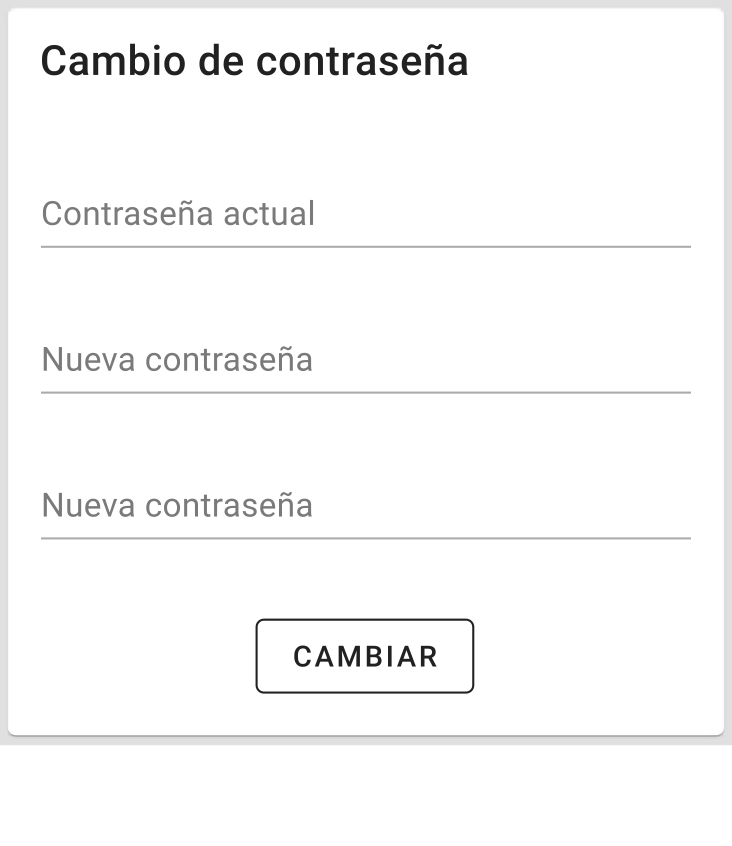
\includegraphics[width=\textwidth]{images/app/change-psw-def.png}
        \caption{Vista de cambio de contraseña por defecto \newline}
        \label{fig:app-change-psw_default}
    \end{subfigure}
    \hfill
    \begin{subfigure}[b]{0.45\textwidth}
        \centering
        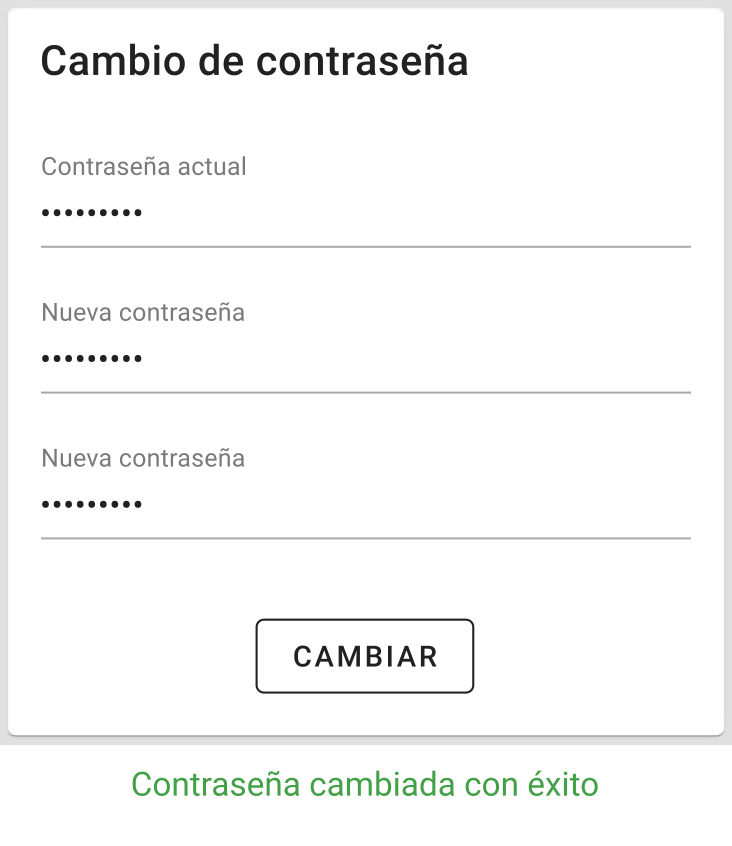
\includegraphics[width=\textwidth]{images/app/change-psw-sucess.png}
        \caption{Vista de cambio de contraseña realizado con exito}
        \label{fig:app-change-psw-success}
    \end{subfigure}
    % \caption{Vista de Cambio de contraseña (I)}
    \label{fig:app-change-psw-1}
\end{figure}
En caso de que la contraseña actual sea incorrecta se mostrará el mensaje de error  \textit{“Contraseña incorrecta”} (Figura~\ref{fig:app-change-psw_error-1}).
En caso de que las contraseñas nuevas no coincidan se mostrará el mensaje de error \textit{“Las contraseñas no coinciden”} (Figura~\ref{fig:app-change-psw_error-2})
\begin{figure}[H]
    \centering
    \begin{subfigure}[b]{0.45\textwidth}
        \centering
        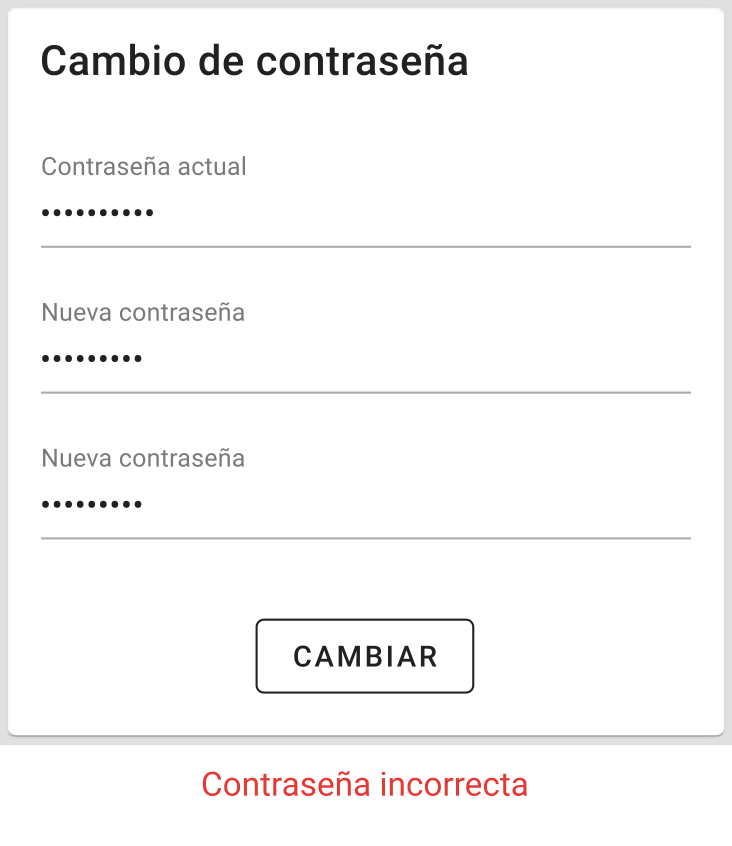
\includegraphics[width=\textwidth]{images/app/change-psw-error1.png}
        \caption{Vista de cambio de contraseña al ingresar contraseña incorrecta}
        \label{fig:app-change-psw_error-1}
    \end{subfigure}
    \hfill
    \begin{subfigure}[b]{0.45\textwidth}
        \centering
        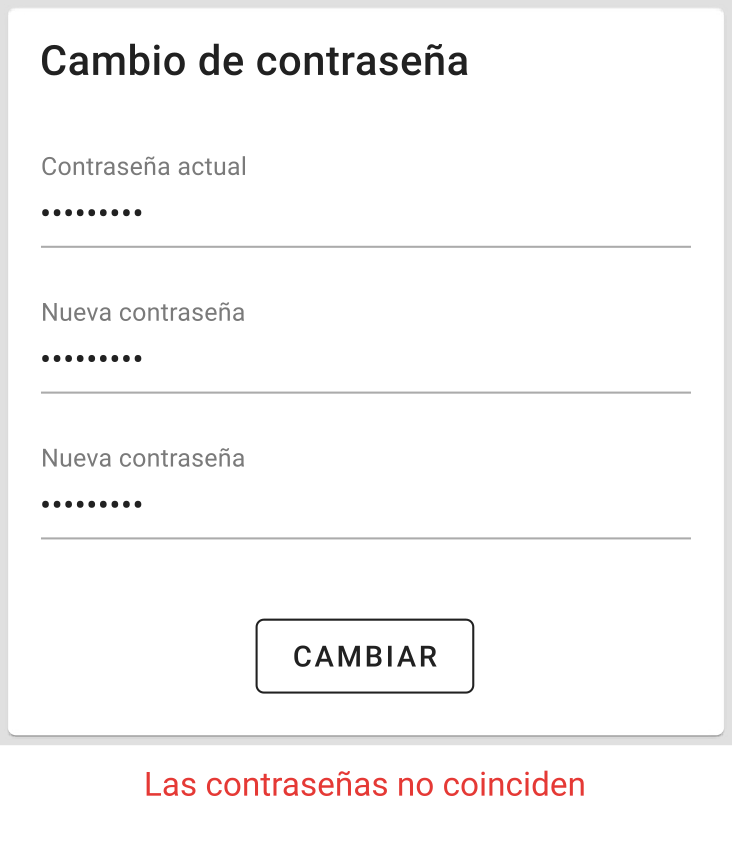
\includegraphics[width=\textwidth]{images/app/change-psw-error2.png}
        \caption{Vista de cambio de contraseña al ingresar contraseñas que no coinciden}
        \label{fig:app-change-psw_error-2}
    \end{subfigure}
    % \caption{Vista de Cambio de contraseña (II)}
    \label{fig:app-change-psw-2}
\end{figure}

En el caso de que la nueva contraseña no cumpla los críterios de seguridad (longitud mínima de 8 caracteres y al menos un número) se mostrará el mensaje de error  \textit{“La contraseña debe tener al menos 8 caracteres / La contraseña debe tener al menos un número”} (Figura~\ref{fig:app-change-psw_error-1}).
\begin{figure}[H]
    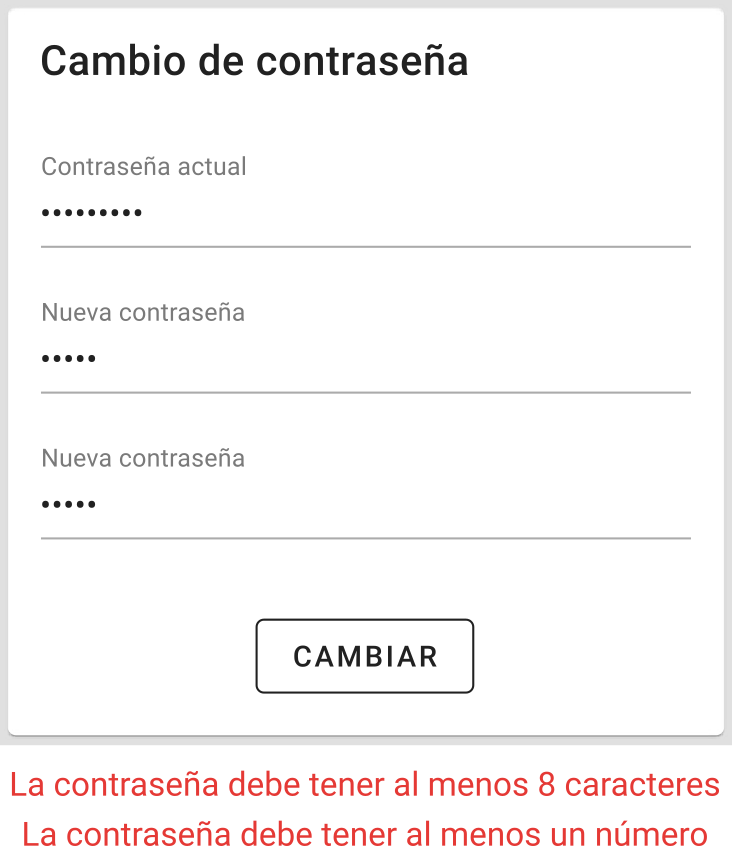
\includegraphics[width=0.45\linewidth]{images/app/change-psw-error3.png}
    \captionsetup{justification=raggedright, width=0.45\linewidth, singlelinecheck=off}

    % \captionsetup{width=0.45\linewidth}
    \caption{Vista de cambio de contraseña al ingresar una nueva contraseña que no cumple con los críterios de seguridad}
    \label{fig:app-change-psw_error-3}
\end{figure}

% \begin{figure}[H]
%     \centering
%     \begin{subfigure}[b]{0.4\textwidth}
%         \centering
%         \includegraphics[width=\textwidth]{images/app/chage-psw-def.png}
%         \caption{a}
%         \label{fig:subfig1}
%     \end{subfigure}
%     \hfill
%     \begin{subfigure}[b]{0.4\textwidth}
%         \centering
%         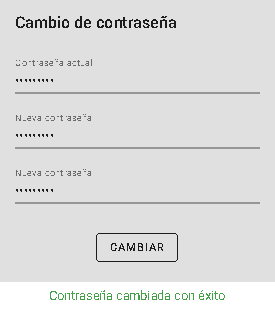
\includegraphics[width=\textwidth]{images/app/chage-psw-sucess.png}
%         \caption{b}
%         \label{fig:subfig2}
%     \end{subfigure}

%     \vskip\baselineskip

%     \begin{subfigure}[b]{0.4\textwidth}
%         \centering
%         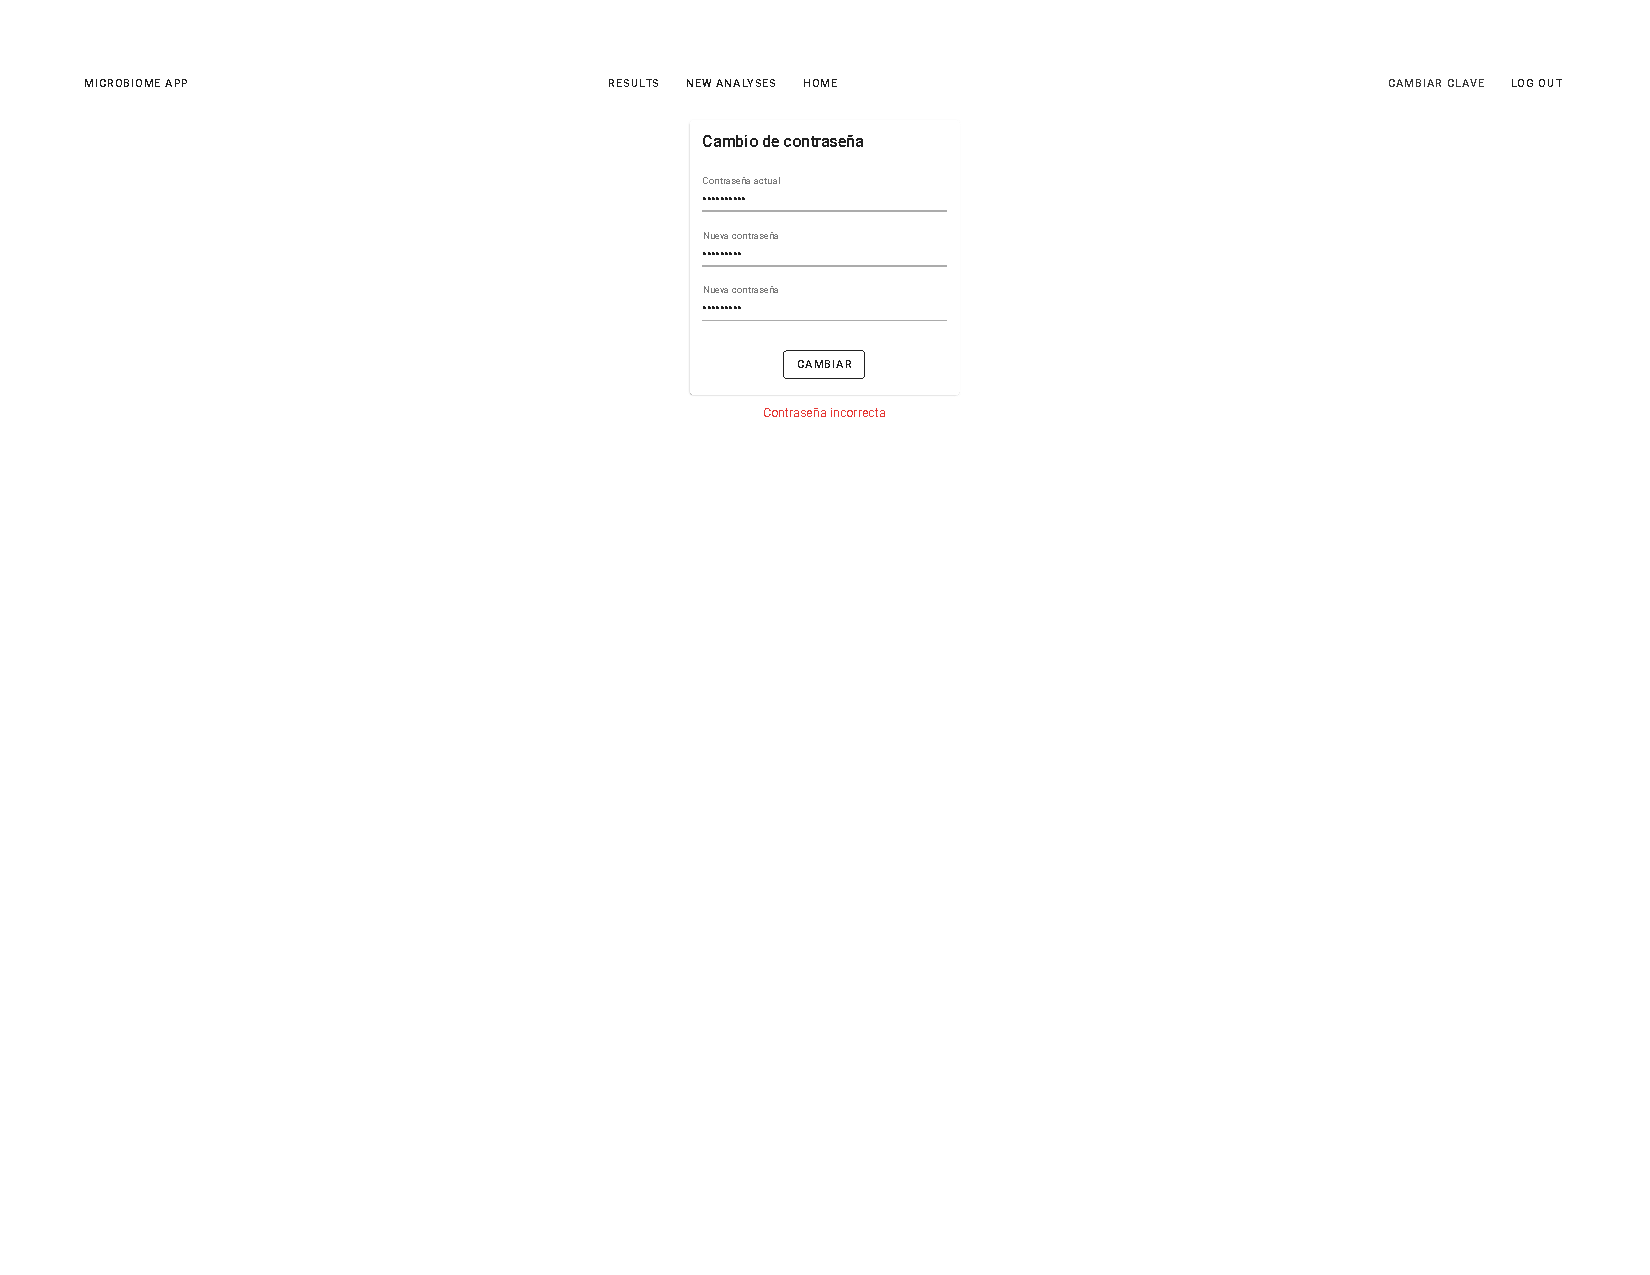
\includegraphics[width=\textwidth]{images/app/chage-psw-error1.png}
%         \caption{c}
%         \label{fig:subfig3}
%     \end{subfigure}
%     \hfill
%     \begin{subfigure}[b]{0.4\textwidth}
%         \centering
%         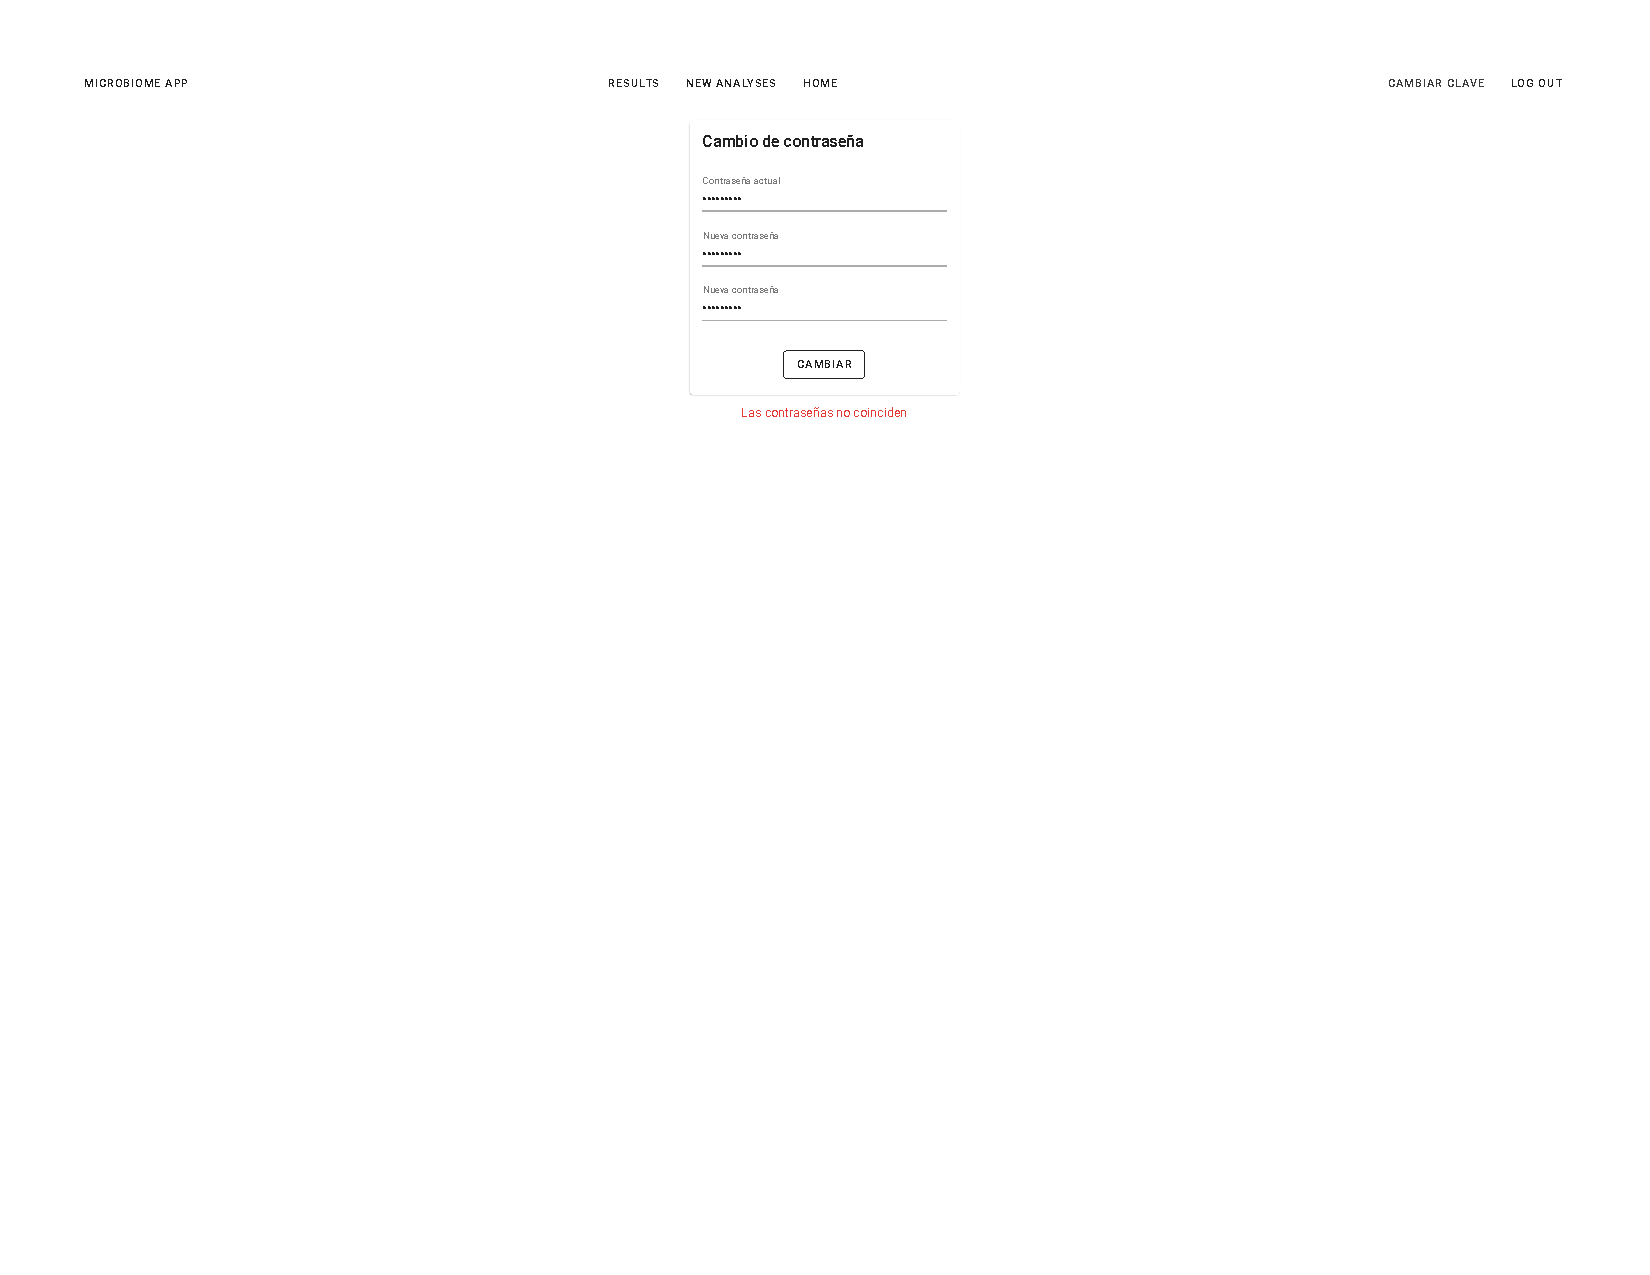
\includegraphics[width=\textwidth]{images/app/chage-psw-error2.png}
%         \caption{d}
%         \label{fig:subfig4}
%     \end{subfigure}

%     \vskip\baselineskip

%     \begin{subfigure}[b]{0.4\textwidth}
%         \centering
%         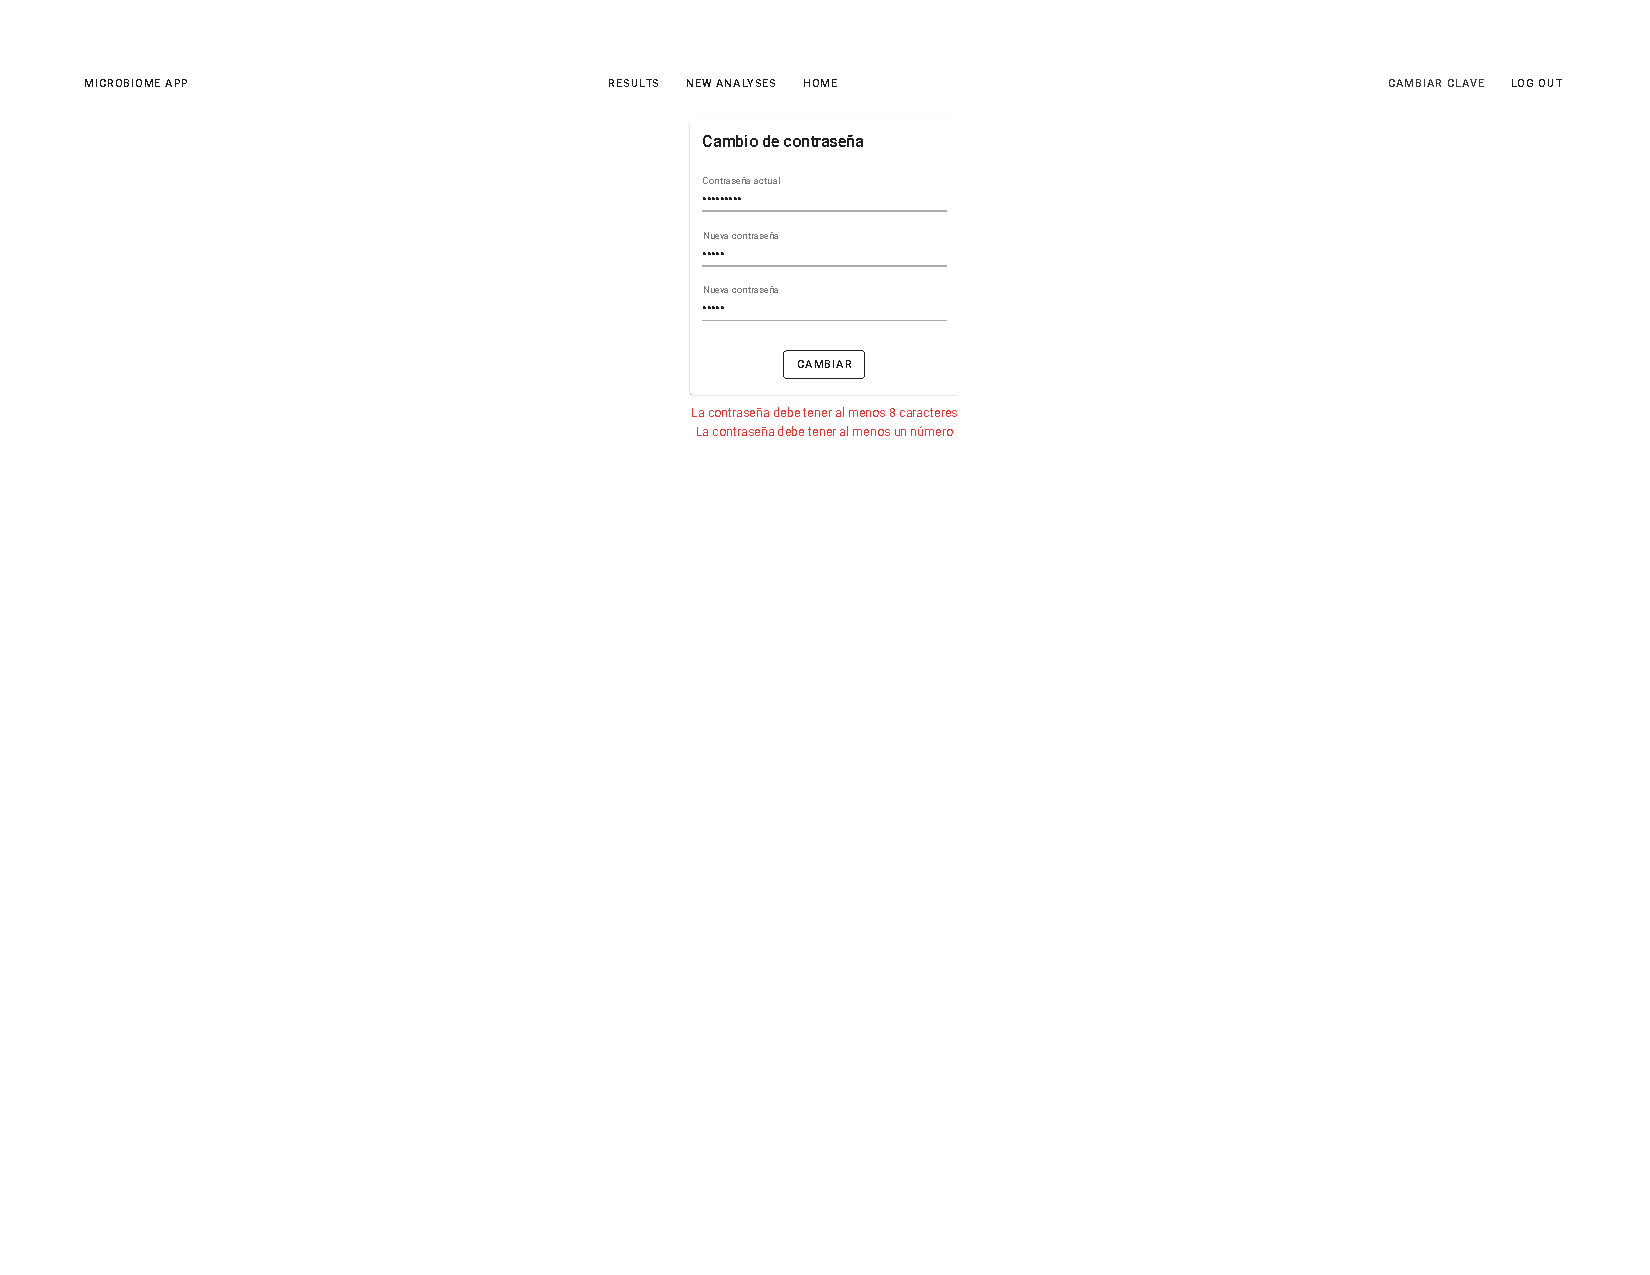
\includegraphics[width=\textwidth]{images/app/chage-psw-error3.png}
%         \caption{e}
%         \label{fig:subfig5}
%     \end{subfigure}
    
%     \caption{Título de la figura principal}
%     \label{fig:main}
% \end{figure}


\subsection{Nuevo análisis}
En esta sección el usuario deberá ingresar la información del proyecto, datos de secuenciación, y metadata para poder realizar los análisis. 
El usuario deberá rellenar la información básica del proyecto como, nombre, descripción, tipo de archivos y mediante un archivo en formato (XLXS) deberá ingresar la información de las muestras. %, como nombre de archivo, nombre de la muestra, barcode (opcional) y grupo (opcional).
Los datos de secuenciación se debe subir a algún directorio del drive del usuario y se debe dar acceso a la cuenta \textit{nanotax.catg@gmail.com}.
La figura~\ref{fig:app-new-analysis-def} presenta la vista inicial de la sección de Nuevo análisis.

\begin{figure}[H]
    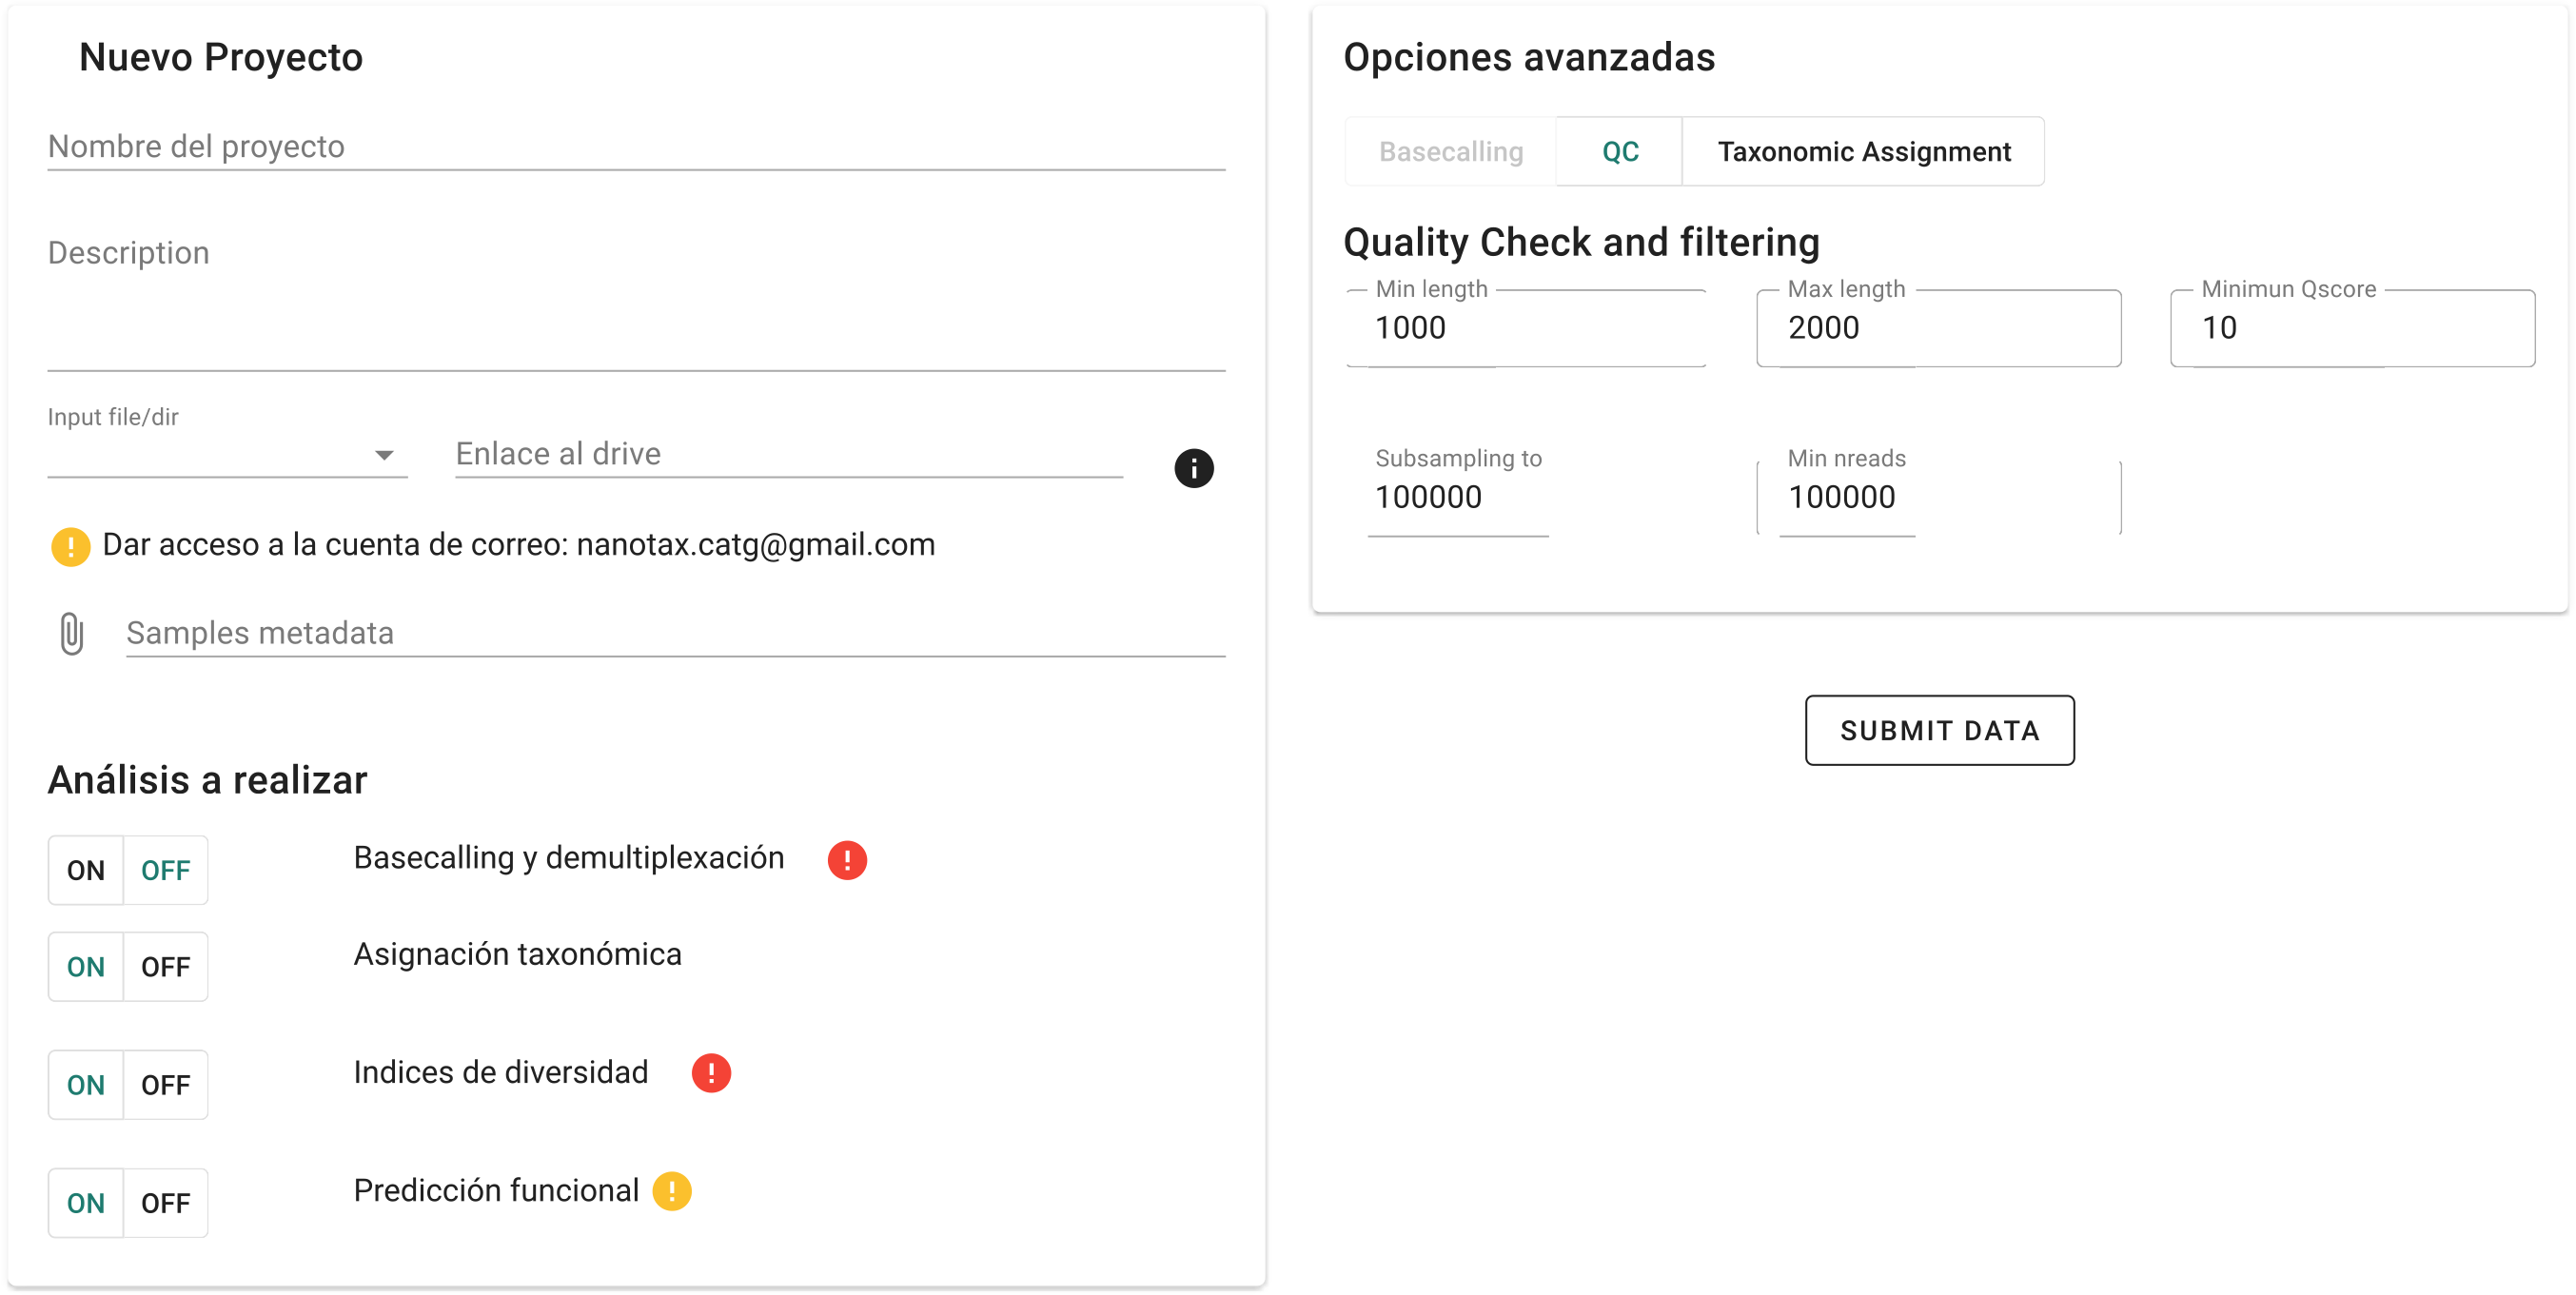
\includegraphics[width=1\linewidth]{images/app/newAnalysis/new-analysis-def.png}
    % \captionsetup{justification=raggedright, width=0.45\linewidth, singlelinecheck=off}

    % \captionsetup{width=0.45\linewidth}
    \caption{Vista por defecto de Nuevo análisis}
    \label{fig:app-new-analysis-def}
\end{figure}


A continuación se describen los datos que el usuario debe rellenar:

\begin{itemize}
    \item Nombre: Nombre del proyecto a utilizar en la plataforma (sección de visualización de proyectos y resultados).
    \item Descripción (opcional): Descripción del proyecto, campo opcional.
    \item Tipo de archivo a subir (POD5, FASTQ): Archivos de secuenciación que se procesarán:
    \begin{itemize}
        \item POD5: En caso de querer comenzar desde el proceso de basecalling y demultiplexación de las muestras.
        \item FASTQ: En caso de querer saltarse el paso de basecalling y demultiplexación e iniciar directamente con el control de calidad y asignación taxonómica.
    \end{itemize}
    \item Archivo de metadata en formato XLXS con las siguientes columnas para cada muestra:
    \begin{itemize}
        \item file: nombre del archivo subido al drive (obligatorio)
        \item sample: identificador de la muestra (obligatorio)
        \item barcode (opcional): barcode que identifica la muestra (en caso de querer realizar basecalling y demultiplexación)
        \item group (opcional): groupo al que pertenece cada muestra (en caso de querer hacer diferenciación entre grupos)
        \item \hl{subgroup: subgrupo al que pertenece cada muestra (en caso de querer hacer diferenciación entre subgrupos)}
    \end{itemize}
    \item Análisis a realizar:
    \begin{itemize}
        \item Basecalling y demultiplexacion
        \item Asignación taxonomica
        \item Indices de diversidad
        \item Predicción funcional
    \end{itemize}
\end{itemize}


En el lado derecho de la vista se puede visualizar una sección de opciones avanzadas, donde el usuario puede modificar los parámetros por defecto en caso de que quiera modificar el comportamiento del pipeline (gigura~\ref{fig:app-new-analysis-def}). Esta información es seleccionados desde la base de datos la cual almacena los parámetros por defecto del flujo de trabajo.

\hl{Cabe destacar que en caso de que el directorio del drive no contenga la información necesaria, el proyecto se subirá correctamente y luego pasara a un estado de datos inválidos }
Los filtros y control de calidad se realizan siempre por lo que no aparecerá la opción en la lista de análisis.
Por defecto basecalling y demuliplexación se encuentra deshabilitado, en caso de que el usuario desee realizar este análisis deberá seleccionarlo, y al hacerlo se desbloqueará la sección de configuración de este análisis (Figura~\ref{fig:app-new-analysis-basecallingON}).



\begin{figure}[H]
    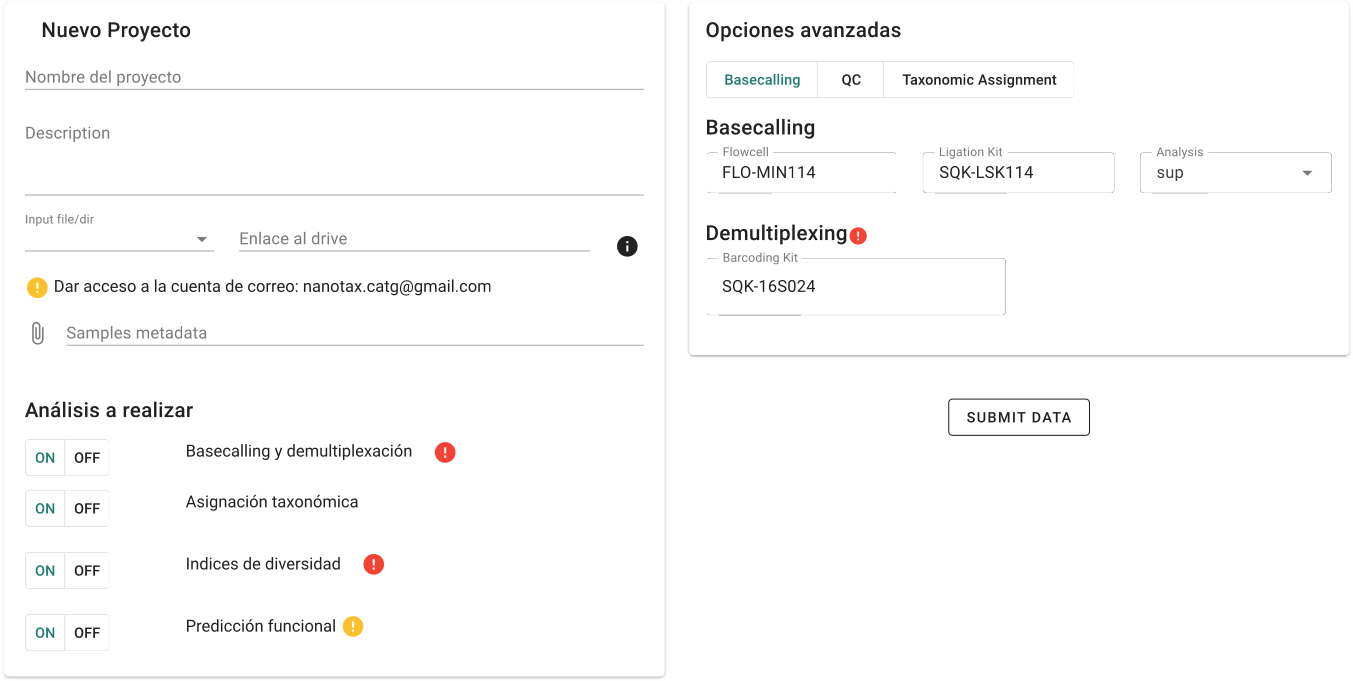
\includegraphics[width=1\linewidth]{images/app/newAnalysis/new-analysis-basecallingON.png}
    % \captionsetup{justification=raggedright, width=0.45\linewidth, singlelinecheck=off}

    % \captionsetup{width=0.45\linewidth}
    \caption{Vista de Nuevo análisis habilitando la opción de basecalling y demultiplexación}
    \label{fig:app-new-analysis-basecallingON}
\end{figure}
% La plataforma se encarga de verificar si el archivo de metadata cuenta con la información necesaria para realizar cada analisis. En caso de que el archivo de metadata no cuente con la información necesaria y el usuario desee realizar uno de esos analisis, se desplegara un mensaje de error al lado del análisis indicando que información se debe añadir en el archivo de metadata. Los parámetros que se pueden modificar son los siguientes:
% \begin{itemize}
%     \item Basecalling y demultiplexacion: Flowcell, kit de ligación y kit de barcoding utilizados durante la secuenciación. Modelo a utilizar para realizar el basecalling
%     \item QC: Longitud mínima y máxima en pares de bases de las lecturas, calidad mínima de las lecturas y cantidad de lecturas a utilizar para los análisis posteriores(subsampleo).
%     \item Predicción funcional: \hl{completar}
% \end{itemize}

% En la parte derecha del componente el usuario puede visualizar los parámetros por defecto y modificarlos en caso de que lo desee. 


Una vez que el usuario presione al botón \textit{Subir proyecto}, la plataforma realiza un proceso de validación para verificar que toda la información subida por el usuario sea correcta. En caso de no serla, la plataforma no permitirá subir el proyecto y podrá presentar alguno de los siguientes mensajes de error:
\begin{itemize}
    \item En caso de no completar el nombre del proyecto o el enlace al directorio del drive ambos campos pasarán a estar en color rojo (figura ~\ref{fig:app-new-analysis-type-file-error}).
    \item En caso de no seleccionar el tipo de archivo a subir, este campo pasará a estar en color rojo y se presentará el siguiente mensaje: \textit{Debe seleccionar el formato de los archivos de entrada} (figura ~\ref{fig:app-new-analysis-type-file-error}).
    \item En caso de seleccionar el formato de archivo \textit{POD5} y no haber seleccionado el proceso de basecalling y demultiplexación como inicio se presentará el mensaje: \textit{Al iniciar con basecalling debe subir los archivos POD5} (figura ~\ref{fig:app-new-analysis-type-file-error}).
    \item En caso de seleccionar el formato de archivo \textit{FASTQ} y haber seleccionado el proceso de basecalling y demultiplexación como inicio se presentará el mensaje: \textit{Al iniciar con QC o asignación taxonómica debe subir los archivos FASTQ} (figura ~\ref{fig:app-new-analysis-type-file-error}).
    \item En caso de que el archivo de metadata no cuente con todas las columnas necesarias se pueden presentar los siguientes mensajes de errores (figura ~\ref{fig:app-new-analysis-type-file-error}) \hl{no todos, solo lo que falte}:
    \begin{itemize}
        \item \textit{El archivo de metadata le falta la columna file}
        \item \textit{El archivo de metadata le falta la columna sample}
        \item \textit{El archivo de metadata le falta la columna barcode}: Solo en caso de seleccionar basecalling y demultiplexación como inicio del pipeline.
        \item \textit{El archivo de metadata le falta la columna group}: Solo en caso de querer realizar análisis por grupos (índices de diversidad).

    \end{itemize}
\end{itemize}


\begin{figure}[H]
    \centering
    \begin{subfigure}[b]{0.45\textwidth}
        \centering
        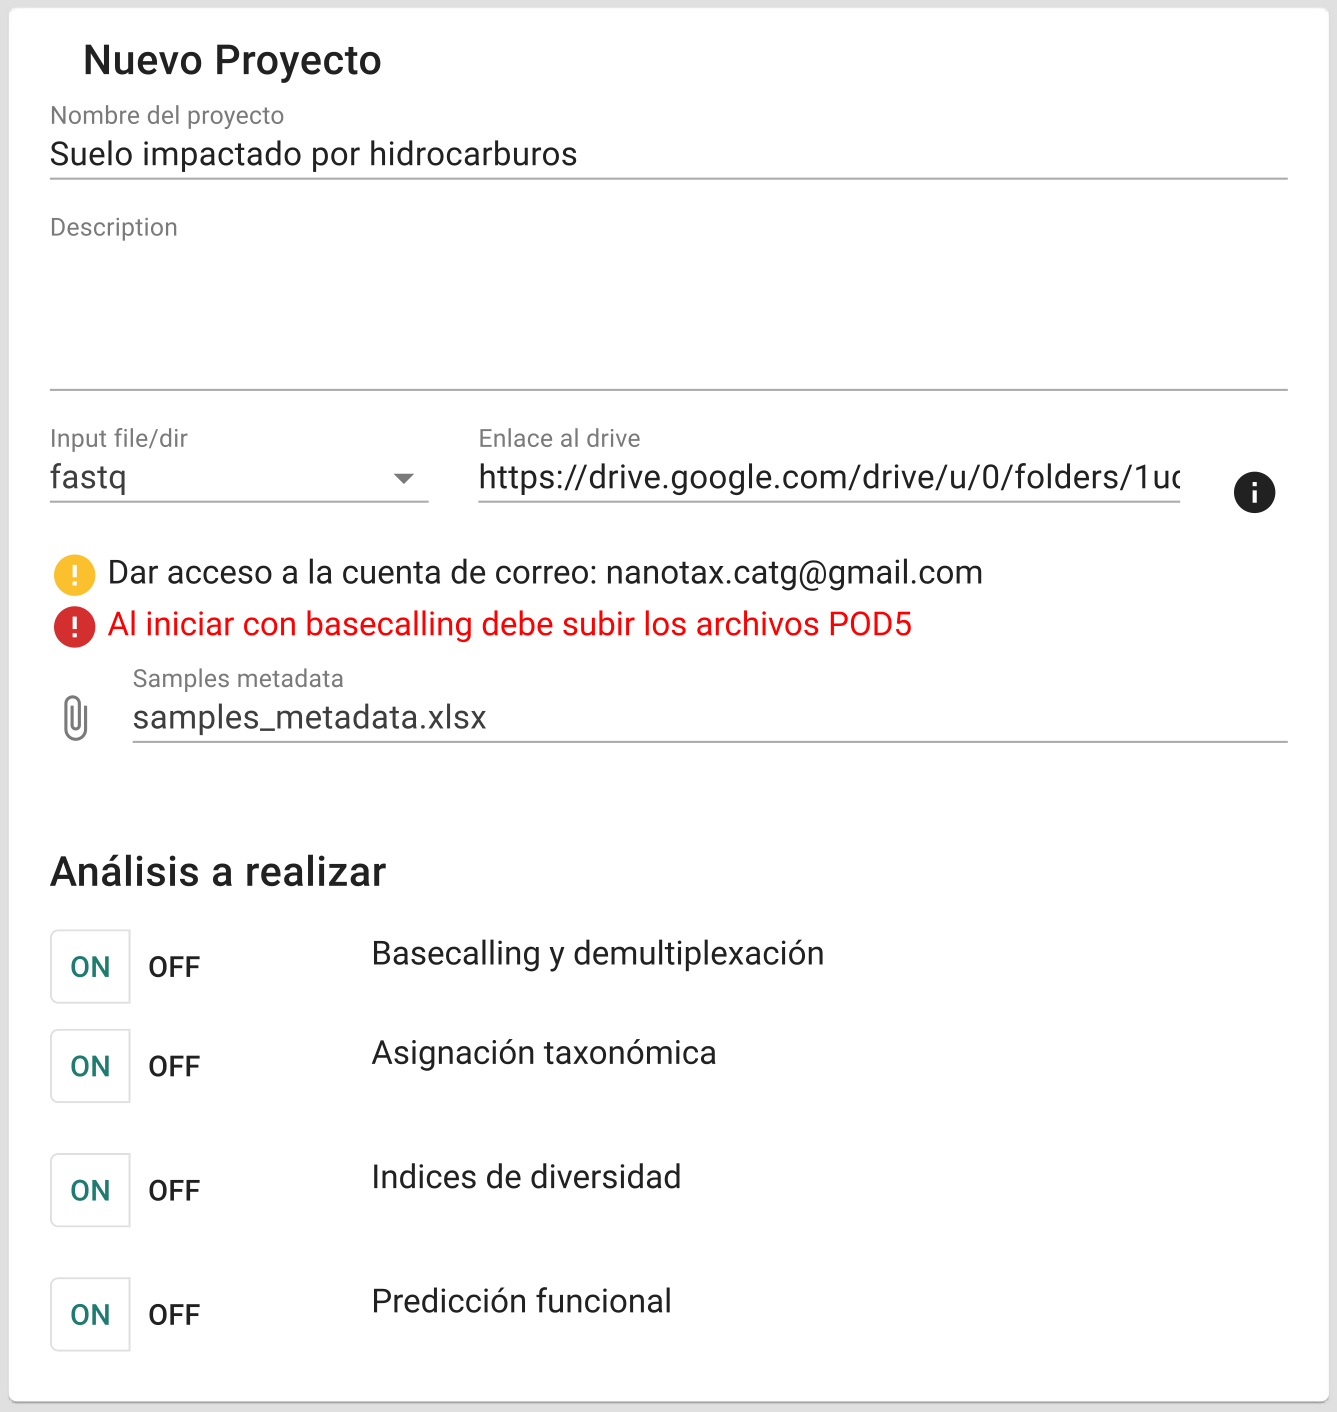
\includegraphics[width=\textwidth]{images/app/newAnalysis/pod5-error.png}
        \caption{Vista de nuevo análisis: Error al seleccionar el tipo del archivo}
        \label{fig:app-new-analysis-pod5-error}
    \end{subfigure}
    \hfill
    \begin{subfigure}[b]{0.45\textwidth}
        \centering
        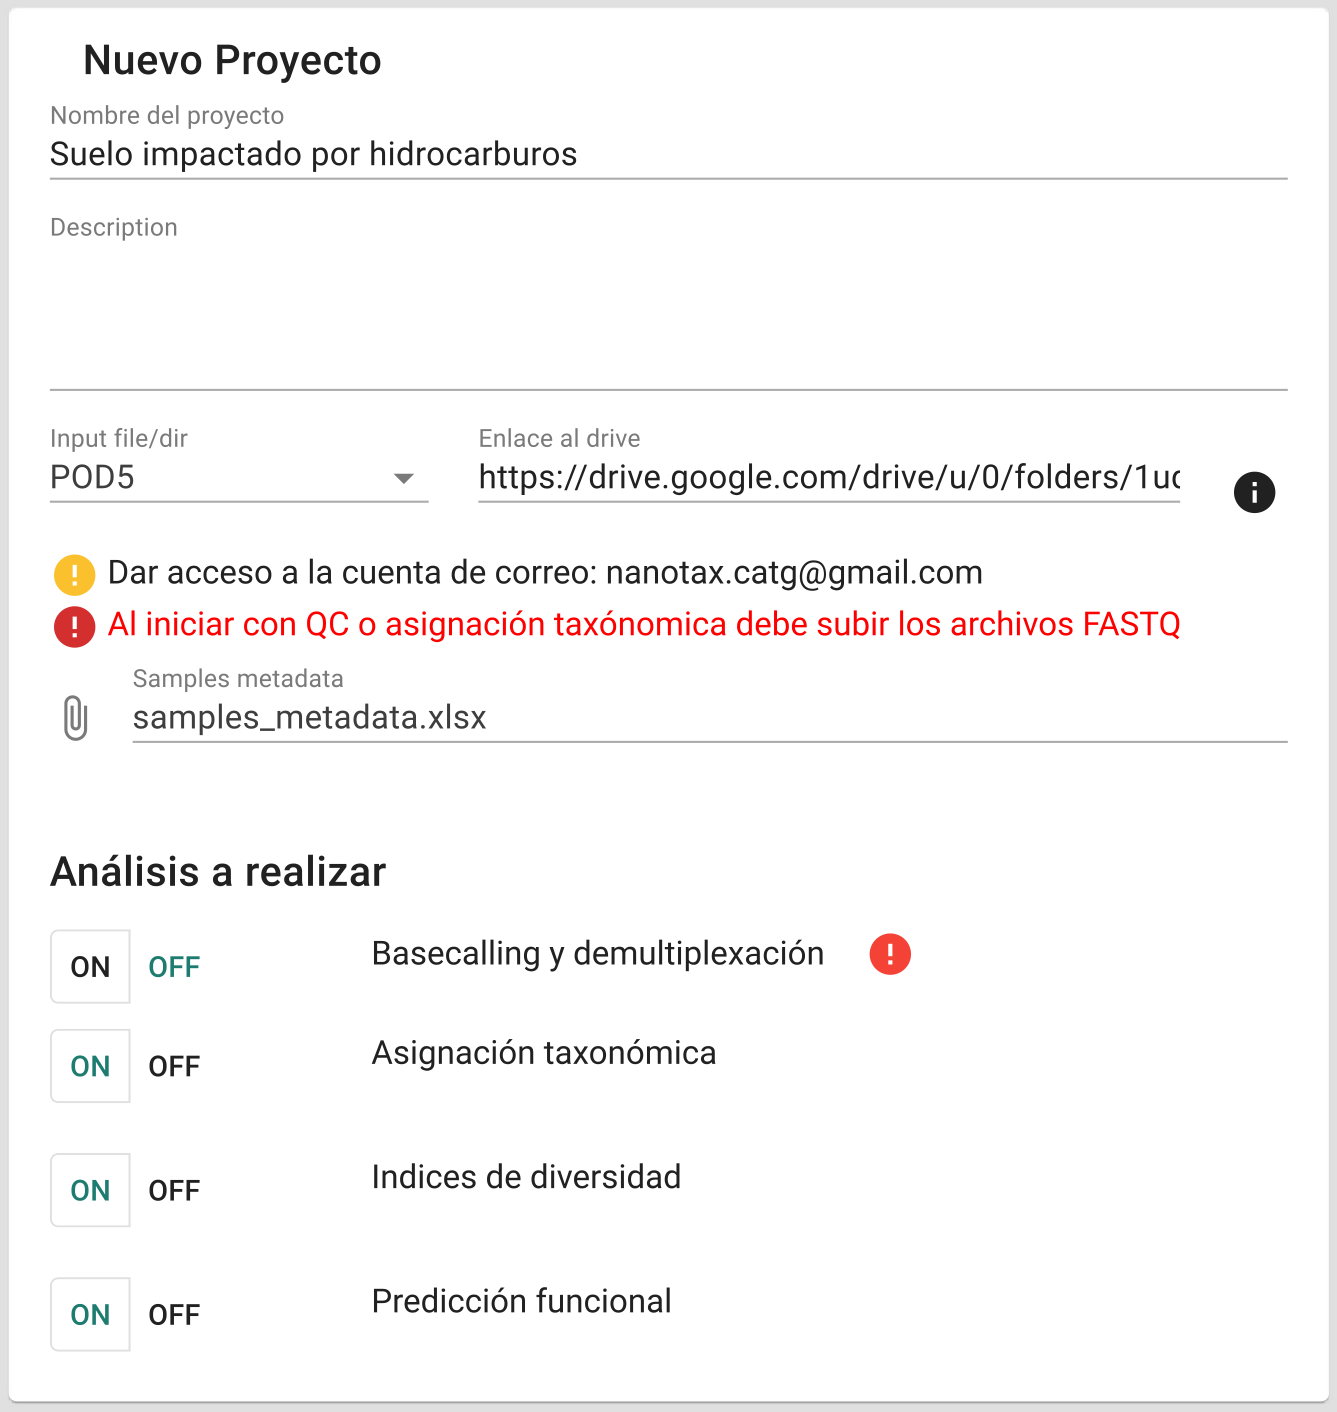
\includegraphics[width=\textwidth]{images/app/newAnalysis/fastq.png}
        \caption{Vista de nuevo análisis: Error al seleccionar el tipo del archivo}
        \label{fig:app-new-analysis-fastq-error}
    \end{subfigure}
    \caption{Vista de nuevo análisis: Error al seleccionar el tipo del archivo}
    \label{fig:app-new-analysis-type-file-error}
\end{figure}



\begin{figure}[H]
    \centering
    \begin{subfigure}[b]{0.45\textwidth}
        \centering
        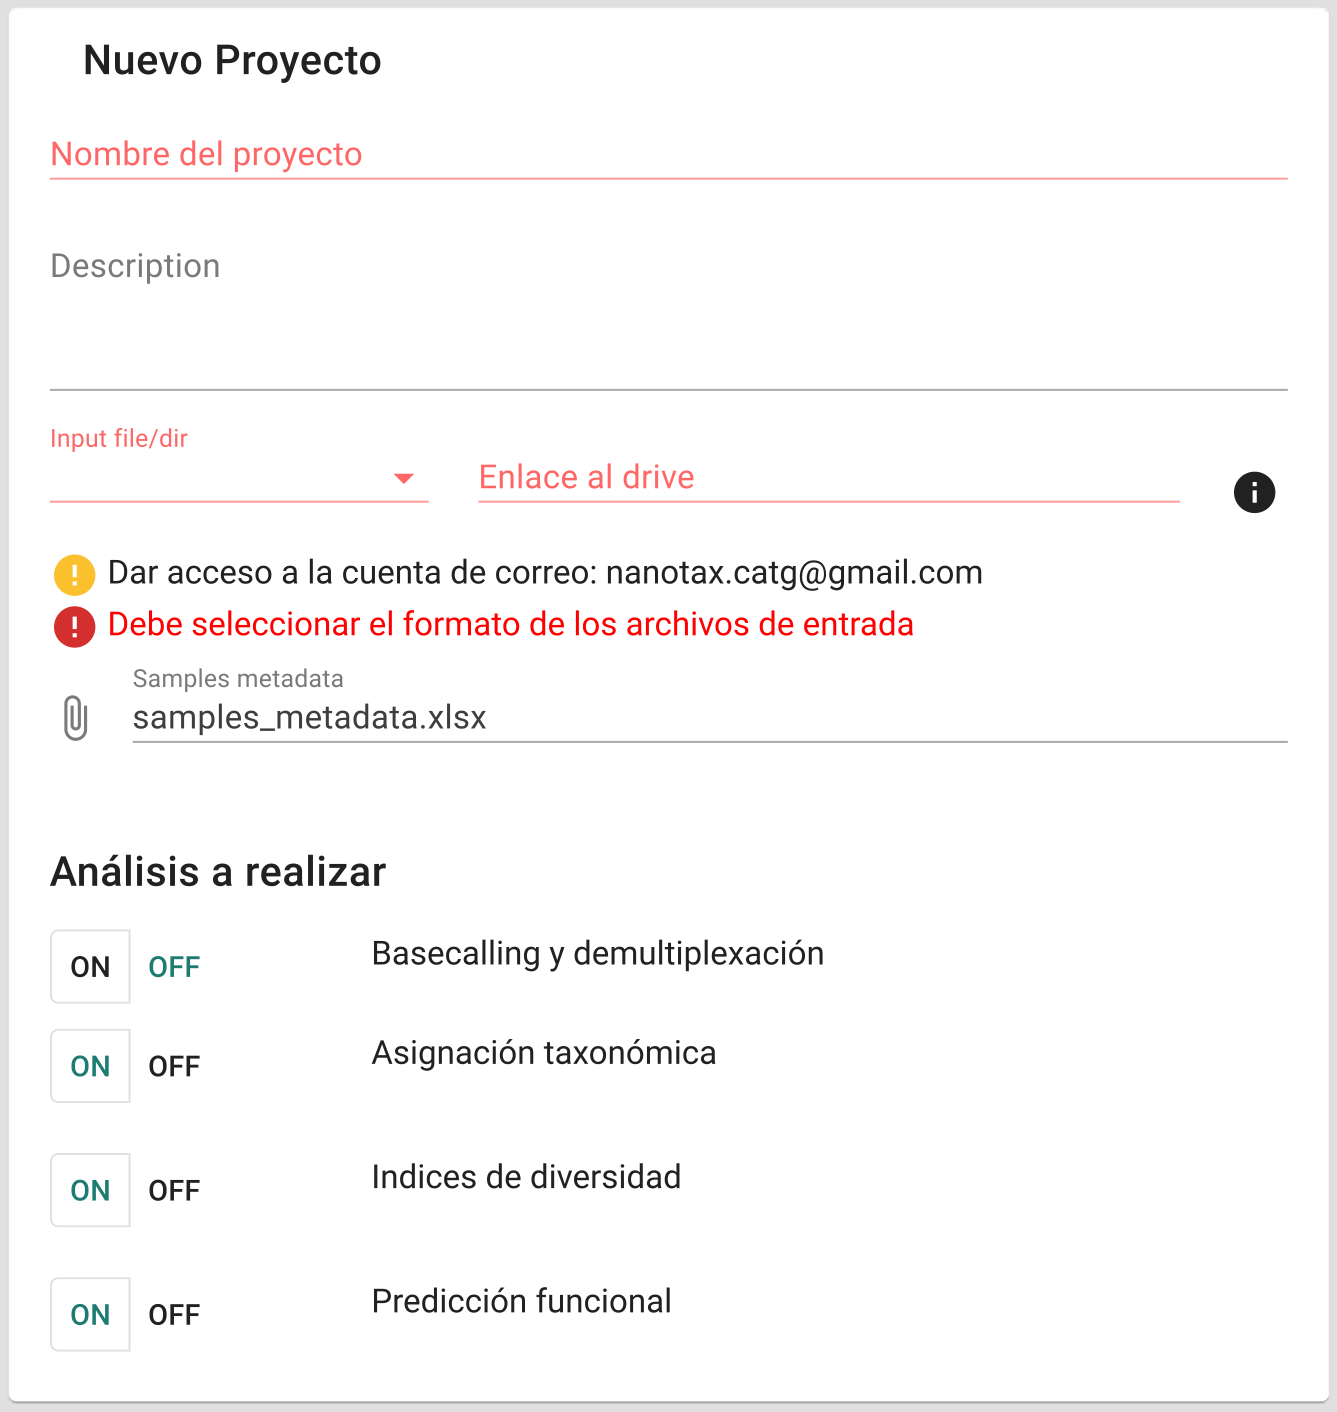
\includegraphics[width=\textwidth]{images/app/newAnalysis/errors1.png}
        \caption{Vista de nuevo análisis: Errores por falta de información}
        \label{fig:app-new-analysis-nodata-error}
    \end{subfigure}
    \hfill
    \begin{subfigure}[b]{0.45\textwidth}
        \centering
        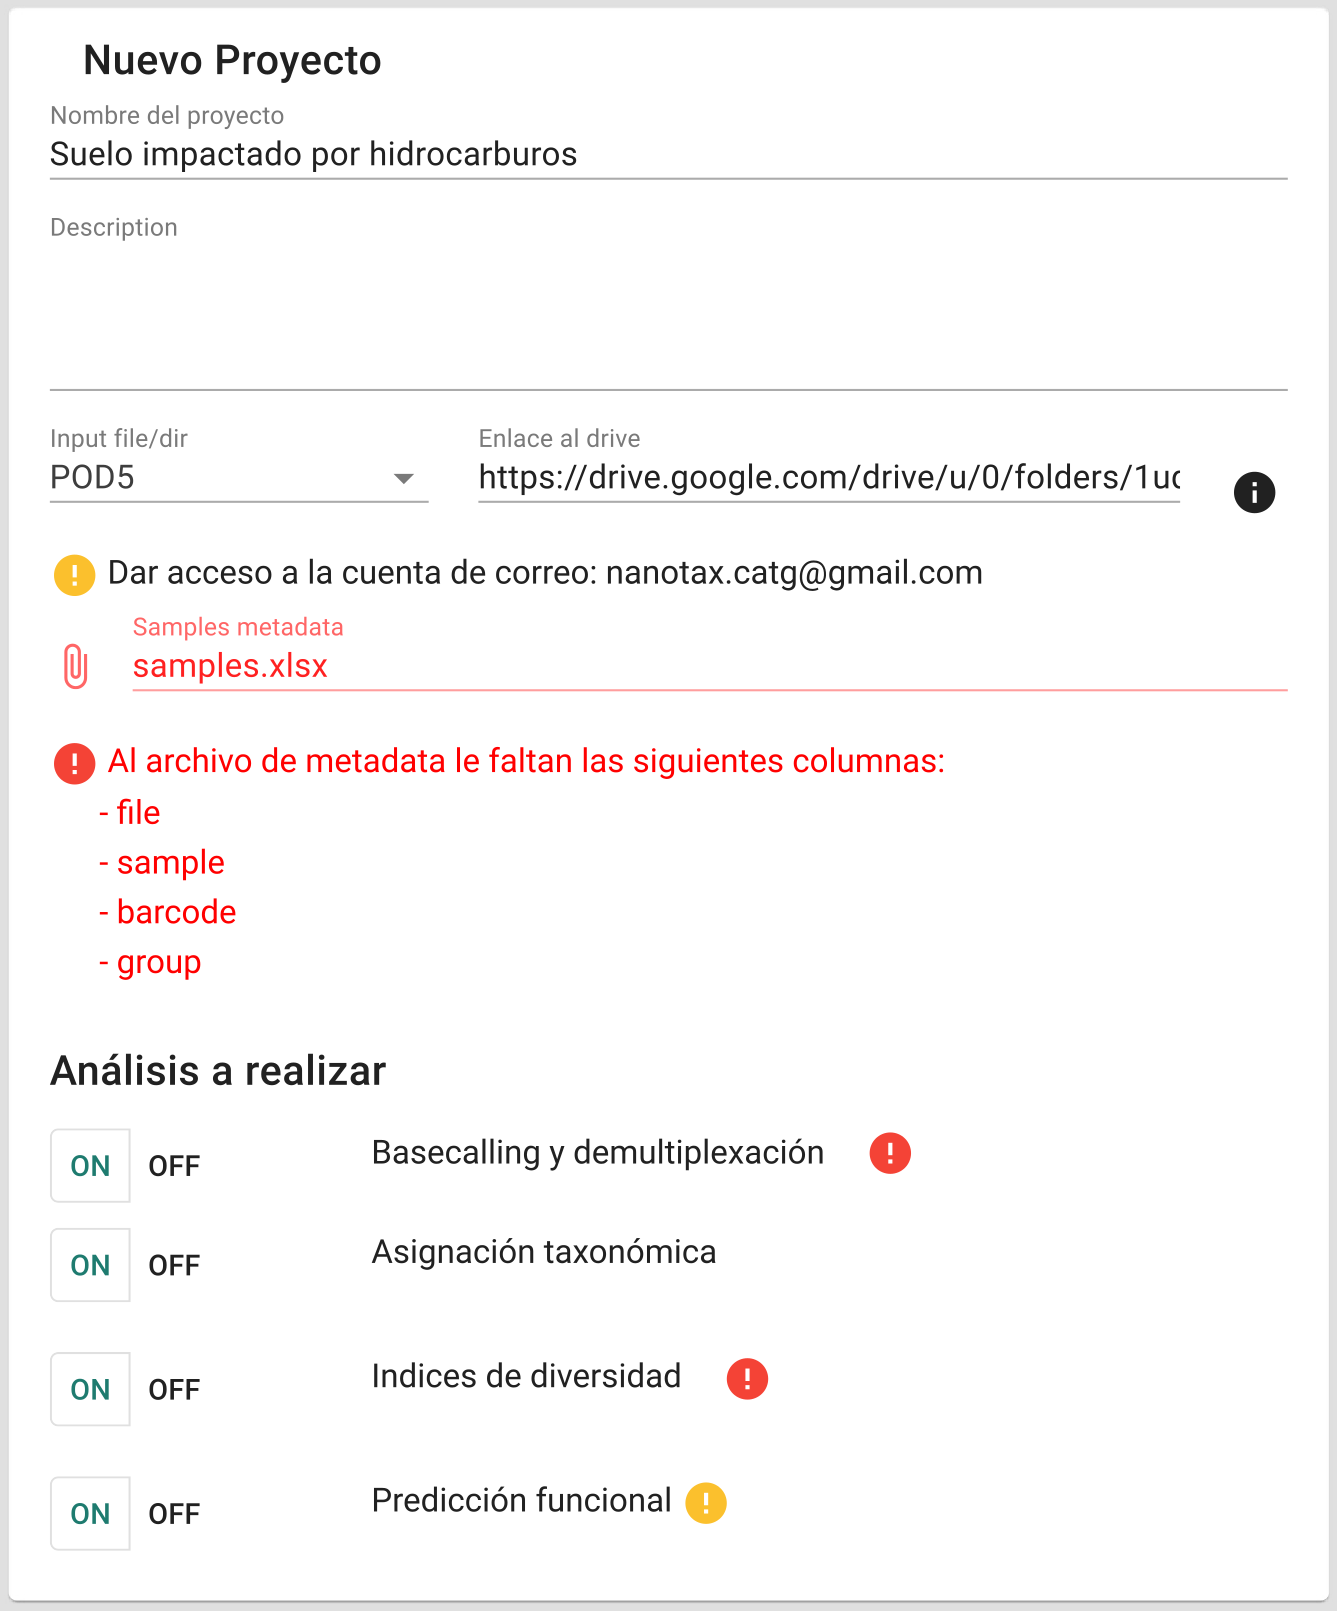
\includegraphics[width=\textwidth]{images/app/newAnalysis/metadata-error-1.png}
        \caption{Vista de nuevo análisis: Errores en el archivo de metadata}
        \label{fig:app-new-analysis-metadata-error}
    \end{subfigure}
    \caption{Vista de nuevo análisis: Errores }
    \label{fig:app-new-analysis-metadata-nodata-error}
\end{figure}









%%%%%%%%%%%%%%%%%%%%%%%%%%%%%%%%%%%%%%%%%%%%%%%%%%%%%%%%%%%%%%%%%%%%%%

\subsection{Resultados/Proyectos} \label{projects}
Una vez que el usuario valida sus credenciales en la plataforma será redireccionado a la sección de Resultados. En esta sección se mostraran los proyectos que el usuario ha subido a la plataforma, estos proyectos pueden estar en ejecución, finalizados o finalizados con errores. 
Por cada proyecto se desplegará la información básica en una tarjeta:
\begin{itemize}
    \item Nombre del proyecto
    \item Descripción del proyecto
    \item Cantidad de muestras procesadas, descartadas y totales
    \item Estado del proyecto (upload\_data / running / failed / finish)
    \item En caso de que el proyecto haya finalizado el usuario podrá acceder a la sección especifica de resultados del proyecto mediante el botón de Ver resultados.
\end{itemize}



En la parte inferior del componente se encuentra el botón de Subir data, el cual al hacer click en el, ingresará la información a la base de datos y copiará los archivos a la plataforma de computo. Una vez que el usuario presionar el botón de subir data, la plataforma se encarga de verificar que se cuente con toda la información necesaria para correr el pipeline.
\subsection{Resultados de un proyecto en especifico}
Una vez que el pipeline haya finalizado su ejecución, la plataforma leerá los resultados desde la base de datos y desplegará la información en la sección de resultados de un proyecto en especifico. Esta sección cuenta con 5 subsecciones, cada una con información específica del análisis realizado. En caso de que al ingresar el proyecto el usuario no seleccione todos los análisis a ejecutar, solo se mostrarán las secciones indicadas por el usuario.

\hl{De que muestras puedo poner información en mi tesis?}
\subsubsection{Informacion Basica de las muestras}
Esta sección se mostrará siempre que el usuario empiece con archivos POD5 o FastQ, es decir, ya sea comenzando el análisis desde el basecalling o desde el control de calidad. \hl{Igual si es que solo se hace asignaicón taxonomica}.

Al lado izquiero del componente se puede visualizar una tabla con la información básica de cada muestra:
\begin{itemize}
    \item Nombre de la muestra
    \item Total de lecturas
    \item Calidad promedio
    \item Largo promedio
    \item Total de lecturas después del control de calidad
    \item Nota (en caso de que la muestra haya sido descartada se indica en esta columna)
\end{itemize}
En la parte inferior de la tabla hay una nota que indica la cantidad de lecturas que se consideraron para los análisis posteriores (subsampleo).

En la parte derecha de la sección se puede visualizar un heatmap donde en el eje X se encuentra el tamaño de las lecturas, y en el eje Y la calidad. El color indica la cantidad de lecturas que se encuentran en esa intersección, mientras más azul, más lecturas tienen la calidad y tamaño indicado.
Para este grafico se consideraron todas las muestras con sus lecturas \hl{antes de los filtros de calidad o después?}.

En la parte inferior del gráfico hay una nota que indica la cantidad de lecturas que se encuentran en un rango especifico. \hl{Este valor es variable ......}
\subsection{Asignación taxonómica}
La sección de assignación taxonómica cuenta con un gráfico de barras apiladas y una tabla por cada categoría taxonómica (especie, genero,  familia, orden, clase y filo).
En la leyenda del gráfico de barras apiladas solo se muestran las 10 taxonomías con mayor abundancia. El usuario puede moverse através del gráfico y posicionarse en las barras para poder visualizar el nombre de la taxonomía y el porcentaje o cantidad de lecturas en una muestra en especifico. Todas aquellas taxonomías que tienen un porcentaje menor a un 1\% (valor por defecto) son agrupadas en una nueva taxonomia llamada \textit{Otros}.
En la parte superior de la tabla se encuentra un campo de texto donde el usuario puede buscar una taxonomía en especifico y visualizar su abundancia o cantidad de lecturas en todas las muestras.

El usuario puede visualizar la información en porcentaje o en cantidad de lecturas manipulando el boton de la parte inferior del gráfico. Asi también puede modificar el porcentaje utilizado para generar la taxonomía Otros.

En caso de que el usuario al crear el proyecto hubiera ingresado información de los grupos asociados a las muestras, se podrá visualizar un nuevo grupo de botones que permiten al usuario visualizar la información de las taxonomías por grupo o por muestra.
\subsection{Similitud entre las muestras}
En esta sección se puede visualizar un gráfico Sunburst el cual representa las taxonomías compartidas entre una cantidad de muestras especificas. Mientras más grande el anillo en el gráfico, indica que la presencia de esa taxonomía es mayor. Cada nivel de anillo representa una categoria taxonomica, siendo la más interna especie y la más externa filo.
En caso de que el usuario haya ingresado grupos asociados a las muestras, se podrán visualizar más gráficos de Sunburst en la sección, un gráfico por cada grupo. En el caso de que el usuario no haya ingresado grupos, podrá visualizar solamente un gráfico que mostrará las taxomías compartidas entre todas las muestras.

En caso de que un grupo no tenga taxonomías compartidas entre si, se desplegará un mensaje indicando esto.
En la parte inferior del gráfico, al lado derecho de la leyenda se puede visualizar un icono, el cual al posicionarse sobre el, va a mostrar las muestras utilizadas para generar el gráfico.
\subsubsection{Indices de diversidad}
En caso de que el usuario hubiera ingresado grupos al inicio del proyecto, se podrá visualizar tres gráficos boxplot, uno por cada indice de diversidad (Shannon, Simpson y Chao2). En caso de que el usuario no haya ingresado grupos, esta sección no se desplegará en la plataforma.
\subsubsection{Predicción funcional}
En esta sección se presenta una tabla con la información de la predicción funcional obtenida mediante PICRUSt2 (EC, KO y Pathways) para cada muestra. En la parte superior se puede visualizar un campo de texto de búsqueda con el cual el usuario puede filtrar la información de la tabla.

En el lado derecho de la sección, en caso de que el usuario hubiera ingresado grupos, se puede ver un gráfico de barras horizontales que muestra los pathways con diferencias significativas entre los grupos (información obtenida mediante Lefse). En caso de que no se haya ingresado información de grupos, solo se desplegará la tabla.
\subsubsection{Descarga de los resultados}
En la parte superior derecha de la sección de resultados, se encuentra un botón con el texto Download data. Al hacer click en este botón se descargará un archivo comprimido con toda los resultados generados por el pipeline.
\begin{itemize}
    \item CSV de asignación taxonomica por muestra y por grupo (en caso de ingresarse), y por porcentaje y cantidad de lecturas
    \item CSV de predicción funcional (EC, KO y pathways)
    \item CSV con los valores del calculo de los indices de diversidad
    \item \hl{PDF con los gráficos de barras apiladas, Sunburst y boxplot}
    \item \hl{Archivo de texto con la información del pipeline (versión, parámetros, etc)}
\end{itemize}
\hl{graficos, csv, información de las bds y versión del pipeline}
\subsection{Documentación}
En esta sección se despliega la documentación del pipeline, la cual cuenta con la información de los módulos, parámetros y herramientas utilizadas en el pipeline. La documentación se encuentra dividida por cada módulo, donde se muestra la versión de la herramienta utilizada y los parámetros por defecto y modificables por el usuario.
\subsubsection{Basecalling y demultiplexación}
\subsubsection{Control de calidad}
\subsubsection{Asignación taxonómica}
\subsubsection{Predicción funcional}
\subsubsection{Indices de diversidad}

